%%%%%%%%%%%%%%%%%%%%%%%%%%%%%%%%%%%%%%%%%%%%%%%%%%%%%%%%%%%%%%%%%%%%%%%%%%%%%%%%
%%%%%%%%%%%%%%%%%%%%%%%%%%%%% IMPORTS AND SETTINGS %%%%%%%%%%%%%%%%%%%%%%%%%%%%%
%%%%%%%%%%%%%%%%%%%%%%%%%%%%%%%%%%%%%%%%%%%%%%%%%%%%%%%%%%%%%%%%%%%%%%%%%%%%%%%%

% General settings
\documentclass[11pt,a4paper,notitlepage]{article}

% Misc includes
\usepackage{array}
\usepackage{xcolor}
\usepackage{longtable}

% For title + abstract page
\usepackage{titling}

% For table of contents with links
\usepackage{hyperref}
\hypersetup
{
    colorlinks,
    citecolor=black,
    filecolor=black,
    linkcolor=black,
    urlcolor=blue
}
\usepackage{ulem}

% For images
\usepackage{graphicx}
\usepackage{subfig}

% For quotes
\usepackage[english]{babel}
\usepackage[autostyle, english = american]{csquotes}
\MakeOuterQuote{"}

% For including code
\usepackage{listings}
\usepackage{color}
\definecolor{dkgreen}{rgb}{0,0.6,0}
\definecolor{gray}{rgb}{0.5,0.5,0.5}
\definecolor{mauve}{rgb}{0.58,0,0.82}
\lstset{
  language=Java,
  aboveskip=3mm,
  belowskip=3mm,
  showstringspaces=false,
  columns=flexible,
  basicstyle={\small\ttfamily},
  numbers=none,
  numberstyle=\tiny\color{gray},
  keywordstyle=\color{blue},
  commentstyle=\color{dkgreen},
  stringstyle=\color{mauve},
  breaklines=true,
  breakatwhitespace=true,
  tabsize=3,
  %frame=single,
  rulesepcolor=\color{gray},
  rulecolor=\color{black}
}

% Math
\usepackage{amssymb,amsmath}
\setlength{\thinmuskip}{3\thinmuskip}
\setlength{\medmuskip}{3\medmuskip}
\setlength{\thickmuskip}{3\thickmuskip}

% For fix notes
\usepackage[english, status=draft]{fixme}
\fxusetheme{color}

% Document title data
\title{\Large{TODO\\2015-2016}\\\Huge{TODO}}
\author{836897 Simone Graziussi}
\date{TODO}



%%%%%%%%%%%%%%%%%%%%%%%%%%%%%%%%%%%%%%%%%%%%%%%%%%%%%%%%%%%%%%%%%%%%%%%%%%%%%%%%
%%%%%%%%%%%%%%%%%%%%%%%%%%%%%%%% DOCUMENT START %%%%%%%%%%%%%%%%%%%%%%%%%%%%%%%%
%%%%%%%%%%%%%%%%%%%%%%%%%%%%%%%%%%%%%%%%%%%%%%%%%%%%%%%%%%%%%%%%%%%%%%%%%%%%%%%%

\begin{document}

\sloppy

%............................................................................%
%................................ TITLE PAGE ................................%
%............................................................................%

\begin{titlingpage}
    \maketitle
    \begin{abstract}
        \large{TODO}
    \end{abstract}
\end{titlingpage}


%..............................................................................%
%............................. TABLE OF CONTENTS ..............................%
%..............................................................................%

\newpage
\tableofcontents
\newpage


%..............................................................................%
%................................... INTRO ....................................%
%..............................................................................%

\part{Introduction}

\section{Context}
Mobile market is continuously expanding, in 2016 2 billion people world-wide own a smarphone and stores like Google Play and Apple's App Store host more than 2 million applications~\cite{stats}.\medskip \\
Due to this widespread, mobile applications require high quality standards and the only way a developer can obtain confidence of correctness and usability in a set of specific circumstances is testing.\bigskip \\
Mobile testing, however, presents several challenges. The main problem is diversity: there are hundreds of different devices that may run an application, each with different hardware capabilities, screen sizes, available sensors and input methods, operative systems or versions of the same operative system. Other issues are for example network availability, internationalization, scripting (e.g. emulate touchscreen gestures during a test) and usability.
\bigskip \\
This thesis focuses on two particular challenges of mobile development:
\begin{itemize}
	\item Events: mobile applications are characterized by a highly dynamic environment, where hundreds of events may be processed every minute, such as sensor data, connectivity changes, user input, network responses, etc. These events can happen in many different orders and frequencies, and, if the developer does not handle them correctly, this may lead to unexpected behaviors or crashes.
	\item Lifecycle: application components are characterized by their lifecycle, i.e. by several working states such as running, paused, destroyed, etc. This particular type of events need to be carefully handled by the developer: for example an application should stop requesting sensor data while paused to avoid wasting resources or to commit unsaved data before it is closed.
\end{itemize}

\section{Objectives}
Given the critical aspects of event concurrency and lifecycle handling mentioned in the previous section, the aim of this thesis is to describe an event-based testing approach for Android applications. The Android operative system was chosen because of its widespread and openness, but the main concepts are valid also for other mobile environments.\bigskip \\
The focus of the first part of the thesis will be on lifeycle changes events. In particular, the problem of lifecycle handling will be addressed first with a static code analysis approach to recognize possible misuses of components, and then with a dynamic approach that will allow the developer to drive the application lifecycle to test its robustness.\bigskip \\
The second part of the thesis will instead focus on generic events, providing to the developer a tool to test their behavior in dynamic conditions. More in detail, a temporal logic language will be defined to specify consistency checks on the stream of events, which will later be implemented in Android exploiting the ReactiveX library, an innovative system of industrial interest.

\section{Achieved Results}
The original contributions of this thesis are:
\begin{itemize}
	\item A survey of some of the approaches to test Android applications, in particular with regard to lifecycle handling and concurrency of events.
	\item A collection of examples of best practices in handling components according to the application lifecycle and the implementation of static checks to help the developer recognize possible misuses.
	\item Implementation of a testing framework that allows to verify the behavior of an application during common lifecycle changes.
	\item Definition of a temporal logic language to describe consistency checks among events and its implementation in a testing tool.
	\item Evaluation... TODO
\end{itemize}

\section{Outline of the Thesis}
The thesis is organized as follows:
\begin{itemize}
	\item Part \ref{part_background} provides background information on testing and Android in general, as a reference to the main concepts used in the document.
	\item Part \ref{part_state_art} analyzes the main technologies available to test Android applications and some examples of research related to the objectives of the thesis.
	\item Part \ref{part_lifecycle} focuses on the lifecycle events and in particular on the static and dynamic approaches to test them.
	\item Part \ref{part_events} explains in detail the concept of event-based testing proposed in the thesis.
	\item Part \ref{part_conclusion} summarizes the main concepts highlighting applicability, limitations and possible improvements.
\end{itemize}


%..............................................................................%
%................................. BACKGROUND .................................%
%..............................................................................%

\part{Background}\label{part_background}

\section{Introduction}
This part introduces more in detail the main concepts that will later be used during the thesis. In particular, it will start with a short description of testing in general, with some terminology that will be employed throughout the thesis. It will then provide some information on Android and its development concepts, with particular attention to component lifecycle, which will be the focus of the first half of the thesis. Finally, it will describe general event-driven systems, introducing some of the issues that will later be addressed by the second half of the thesis.

\section{Testing}
Testing is the process used in software development to assess the validity of functional and non-functional requirements of an application. Although this verification is able to guarantee the correctness of the tested components within the specific conditions described by the test cases, testing cannot assess the validity of the whole application in every situation, because this would require an unfeasible amount of detail. For this reason, testing is mainly used to discover software bugs in particular situations and to reach an acceptable confidence that the program works as expected under the most common conditions.\bigskip \\
Test cases require a mechanism to actually determine the test outcome, i.e. to tell if the application behaves as expected during the validation process. This mechanism, called oracle, should ideally be complete but avoiding over-specification, while also being efficiently checkable~\cite{Baresi:Oracles}. Oracles can assume many forms, for example the behavior of the application is compared with the technical specifications (e.g. documentation), it is automatically checked by the system thanks to some constructs that allow the developer to specify the test conditions or it can even be manually evaluated by a human being.\bigskip \\
Test cases can be designed from different points of view. In particular, we can have:
\begin{itemize}
	\item White-box testing: the focus is on the internal structure of the application, i.e. tests are defined at the source code level (\textit{how} the software behaves).
	\item Black-box testing: examines the external behavior of the application without considering the actual implementation, i.e. tests are defined at the user level (\textit{what} the software does).
	\item Grey-box testing: combination of white-box and black-box testing. Tests are defined with a partial knowledge of the internal structure of the application (i.e. how the main components interact and the general algorithms used).
\end{itemize}\bigskip
There are usually four levels on which test cases can be defined:
\begin{itemize}
	\item Unit Testing: focuses on a specific unit of the program, for example a single function/method/class used in the source code. Usually, it follows a white-box testing approach and it is performed during development to build a program using units guaranteed to work.
	\item Integration Testing: tests interactions between components of the application, i.e. it usually puts together the units tested in the previous step to see if they work well together.
	\item System Testing: it considers the program as a whole to see if it meets all requirements and quality standards.
	\item Acceptance Testing: final step that decides if the application is complete and ready to be deployed (e.g. released to the public).
\end{itemize}

\section{Android}

\subsection{Operative System}
Android is a operating system (OS) developed by Google. It is designed primarily for touchscreen mobile devices like smartphones and tablets, but recently it was extended to televisions (Android TV), cars (Android Auto) and smartwatches (Android Wear).\medskip \\
The OS is a multi-user Linux system in which each app is a different user. It is characterized by the so called sandboxing mechanism: each process runs in its own virtual machine (VM) and so every app runs in isolation from the other applications. This means that, by default, an application can access only a limited set of components, i.e. only the parts of the system for which it has specific permissions.\medskip \\
Android applications are developed in a Java language environment. The Android Software Development Kit (SDK) compiles code, data and resources into a package called APK, which is used by the devices to install the application.

\subsection{Application Components}
Android applications are built by five main components, each with its specific purpose:
\begin{itemize}
	\item Activity: an activity represents a single "action" that the user can take and, since almost all activities interact with the user, they provide a screen with a user interface. Each activity in the application is independent from the others, but it is of course possible to start an activity (for example when the user clicks on a button) from another to build the application flow.
	\item Fragment: this component was introduced in Android 3.0 (API level 11) to support dynamic and flexible UI on large screens, for example on tablets. A Fragment  represents a "portion" of an Activity, with its own state and UI. Each Activity can contain multiple Fragments at a time, Fragments can be added/removed at runtime and each Fragment can be reused in more than one Activity. A Fragment can only be instantiated inside an Activity.
	\item Service: a Service is a component that is executed in background and, as such, it provides no user interface. It is used to perform complex computations or to interact with an external API (e.g. via the network). The advantage of this approach is that another component (e.g. an Activity) can start and interact with a Service in order to avoid blocking its UI with computationally intensive operations.
	\item Content Provider: a content provider allows to store and retrieve data in some persistent storage location, for example a local SQL database or a remote repository. The provided data can be shared among different applications or private to a specific one.
	\item Broadcast Receiver: a Broadcast Receiver responds to global messages, i.e. messages received by all applications on the device. These events may be fired by the system (e.g. the device has just rebooted) or by a single application (e.g. some data is available), and then intercepted by the applications interested to them.
\end{itemize} 
Activities, Services and Broadcast Receivers are started asynchronously by messages called Intents. This allows not only an application to start its own components, but also to call on other applications. For example, a game may start its internal GameService to manage the game loop, but also send an Intent to a social network application to share the game progress.

\subsection{Component Lifecycle}
App components in Android such as Activities, Fragments and Services are characterized by their lifecycle, i.e. the current runtime state. In general each component is started and then destroyed, but some can also be paused and resumed, and go through several other states.\medskip \\
When a lifecycle state transition happens, the Android system allows the developers to implement several callbacks in the component implementation to manage their behavior in those particular situations. In particular, the Java classes that define a component (such as \texttt{Activity}), which are sub-classed by the developer, allow to override one or more methods to handle the callbacks (such as \texttt{onCreate()} or \texttt{onPause()}).

\subsubsection{Activity Lifecycle}
An Activity can be in three static states:
\begin{itemize}
	\item Resumed: the Activity is visible and can receive user input.
	\item Paused: the Activity is \textit{partially} hidden by another visual component, for example a notification dialog, and has lost the focus. When the Activity is paused it cannot receive any user input or execute code.
	\item Stopped: the Activity is completely hidden to the user, i.e. it is in the background. Like in the previous case, the activity cannot receive inputs or run code. In this state the Activity is still "alive": the state (e.g. member variables) is retained and the Activity can be later restarted.
\end{itemize}\medskip
An Activity can also be in two transient states:
\begin{itemize}
	\item Created: the Activity has been instantiated and will soon become Started.
	\item Started: the Activity has been initialized and will soon become Resumed.
\end{itemize}\medskip
Finally, an Activity can be Destroyed. In this "state" the Activity instance is dead. An Activity can for example be destroyed when the user presses the back button or by the OS when it is stopped and the device needs to free resources. In the latter case, if the application is then reopened by the user, the operative system provides a way to restore the lost information: in particular, the developer can override the callbacks \texttt{onSaveInstanceState()} and \texttt{onCreate()} to pass data between the old and the new instance.\bigskip \\
The following image shows a simplified scheme of the Activity lifecycle transitions with the corresponding Java callbacks.
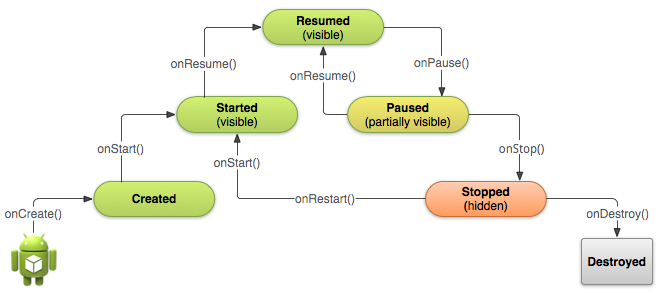
\includegraphics[width=450px]{Images/Android/basic-lifecycle.png}

\subsubsection{Fragment Lifecycle}
The lifecycle of a Fragment is closely related to the lifecycle of the Activity that contains it: for example, when an Activity is paused, all the contained Fragments are paused too. In addition to this, however, Fragments can go through lifecycle changes independently of their host Activity: in particular, since fragments can be dynamically added and removed at runtime, they can be created and destroyed while the Activity is running. Moreover, the developer also has the option to store removed fragments in the so-called backstack and be able to restore them later for example when the user presses the "back" button.\medskip \\
Like Activities, Fragments are characterized by three static states:
\begin{itemize}
	\item Resumed: the Fragment is visible and can receive user input.
	\item Paused: the Activity that contains this Fragment is \textit{partially} hidden by another visual component and has lost the focus.
	\item Stopped: the Fragment is completely hidden to the user. This can happen if the host Activity is also not visible (i.e. in background) or if the Fragment has been stored in the backstack. Like Activities, stopped Fragments are still "alive" and their state is retained.
\end{itemize}
Lifecycle management for Fragments is very similar to the one for Activities, since all callbacks are the same. Fragments provide however some additional methods to manage the interaction with the host Activity: for example \texttt{onAttach()} is called when the Fragment is linked to an Activity, \texttt{onCreateView()} when the Fragment is ready to build its UI, etc.\bigskip \\
The following image shows the main Fragment callbacks:
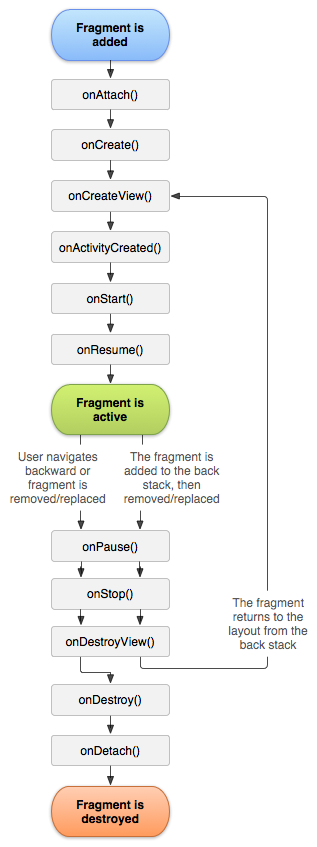
\includegraphics[width=200px]{Images/Android/fragment_lifecycle.png}

\subsubsection{Managing the Lifecycle}\label{managing_lifecycle}
Handling the components lifecycle is a critical aspect in developing an Android application and it is often source of bugs or unexpected behaviors. For example, properly implementing Activity/Fragment lifecycle methods ensures that the app:
\begin{itemize}
	\item Does not waste system resources (e.g. device sensors) while the user is not interacting with it.
	\item Stops its execution when the user leaves the application (for example a game should pause if the user receives a phone call).
	\item Retains its state if the user leaves and then returns to the application (e.g. a messaging app must keep a partially written message even if the user puts the app in background for a moment).
	\item Does not crash or loses user progress when lifecycle changes occur (e.g. an app that does not correctly manage lifecycle may crash with a NullPointerException if some internal component was destroyed during \texttt{onStop()} but not restored during \texttt{onStart()}).
	\item Adapts to configuration changes (like a device rotation between landscape and portrait modes) without losing data or crashing.
\end{itemize}\medskip
In general, for Activities and Fragments the developer should make sure to:
\begin{itemize}
	\item During \texttt{onCreate()}:
	\begin{itemize}
		\item Set the layout resource defining the UI.
		\item Initialize View components (e.g. add click listeners to buttons).
		\item Initialize the component logic (e.g. class-scope variables).
		\item Restore the previous state (if any) saved during \texttt{onSaveInstanceState()} [this can be alternatively performed during \texttt{onRestoreInstanceState()}].
	\end{itemize}
	\item During \texttt{onRestart()}:
	\begin{itemize}
		\item Requery raw Cursor objects previously deactivated during \texttt{onStop()}.
	\end{itemize}
		\item During \texttt{onStart()}:
	\begin{itemize}
		\item Acquire "secondary" resources (e.g. Broadcast Receiver).
		\item Verify system features (e.g. GPS enabled), because they may change when the application is in background.
	\end{itemize}
	\item During \texttt{onResume()}:
	\begin{itemize}
		\item Start animations and similar CPU-intensive operations.
		\item Acquire "critical" resources (e.g. camera, sensors).
		\item Should \textit{not} restart on-going operations that require user visibility (e.g. games, videos), but let the user decide when to do so.
	\end{itemize}
	\item During \texttt{onPause()}:
	\begin{itemize}
		\item Commit unsaved changes made by the user (e.g. save a draft for an unfinished email), if it does not require too much time.
		\item Stop animations and other operations that may be consuming CPU.
		\item Stop on-going operations that require user visibility (e.g. games, videos).
		\item Release "critical" resources (e.g. camera, sensors).
		\item Should \textit{not} perform any long running operation, the call to this method must be very quick.
	\end{itemize}
	\item During \texttt{onStop()}:
	\begin{itemize}
		\item Release "secondary" resources (e.g. Broadcast Receiver).
		\item Perform CPU-intensive shutdown operations (e.g. write unsaved data to database).
	\end{itemize}
	\item During \texttt{onDestroy()}:
	\begin{itemize}
		\item Stop background threads created during \texttt{onCreate()}.
		\item Release long-running resources that could create memory leaks.
		\item Should \textit{not} save data, because the method may not be called in all situations.
	\end{itemize}

\end{itemize}

\section{Event-based Systems}

\subsection{Event-Driven Architecture}
Event-Driven Architecture is a software pattern where the focus is on generation and reaction to events. An event can be defined as a message generated by a producer that represents a change of state or a relevant action performed by some component/actor (e.g. the user). Once generated, events are sent via event channels to all the consumers that are interested to them. Event-Driven Architectures are:
\begin{itemize}
	\item Extremely loosely coupled: the producer does not know about the consequences of its events. It just generates them and then it's up to the consumers to manage everything else.
	\item Well distributed: an event can be anything and exist almost anywhere.
\end{itemize}

\subsection{Android as an Event-Driven Architecture}
Android is implemented as an event-based system. This is because a mobile device must manage several events, like clicks on the touchscreen, sensor data, network requests/responses, etc.\smallskip \\
From an application point of view, events can be generated internally (e.g. from a service/thread created by the application itself) or externally (e.g. sensor data). Each application is composed of several threads, a subset of which, called Looper threads, are in charge of processing events by invoking an appropriate event Handler for each of them.\smallskip \\
Events from a single thread are atomic, i.e. they are placed on a FIFO event queue and processes one by one. However, events produced by several threads are processed concurrently and not guaranteed to be ordered or atomic. For example the user may click on a button while the application receives a network response and the device broadcasts some sensor data.\medskip \\
Examples of events that can be observed in an Android application are:
\begin{itemize}
	\item User input events can be observed attaching listeners to View components. An event listener is a Java interface whose methods are called by the Android framework when the View is triggered by user interaction, for example the \texttt{onClick()} callback of a listener attached to a Button will be called when the user clicks on that button. The developer can then implement the callback to perform any action in response to the input event generation, e.g. starting another activity.
	\item Lifecycle events are triggered when there is a state transition of some component, like an Activity. For example the \texttt{onPause()} callback is invoked when an Activity is paused.
	\item Broadcast events like system messages (e.g. device boot completed, alarm goes off, etc.) or application-specific messages are received by BroadcastReceivers in the \texttt{onReceive()} callback.
	\item Asynchronous messages from services external to the application (e.g. sensor data, network requests, etc.) also have their specific callbacks.
\end{itemize}

\subsection{Event Concurrency Errors}
The concurrency among events inside a single application can lead to unexpected behaviors or crashes.\smallskip \\
When the Android developer decides to explicitly create a multi-threaded application we may have the classical problems of concurrency like synchronization, deadlocks and starvation, but problems arise even if he/she does not manually create threads, due to the aforementioned concurrency of events.\smallskip \\
In this context, the most relevant challenge in an Android application is race conditions: two or more events do not happen in the order the programmer intended. A simple example of this issue is when the developer asynchronously starts an AsyncTask (an utility class that allows to perform short operations in the background without blocking the UI thread) to download an image from the network. The AsyncTask, when the download is completed, expects the Activity that started it to be still there to receive the result, but maybe the user already left the application and so we encounter for example a NullPointerException.


%..............................................................................%
%............................ STATE OF THE ART ................................%
%..............................................................................%


\part{Android Testing State of the Art}\label{part_state_art}

Android tests are mainly based on JUnit~\cite{JUnit}, a testing framework for Java. It allows to create classes called test cases that contain methods annotated with \texttt{@Test}, each representing a test.

\section{Unit Testing}
White-box unit testing in Android can be:
\begin{itemize}
	\item Local: it runs on the local development machine (i.e. the computer where the application is coded). It has the advantage of being fast (avoids the overhead to load the application in a device/emulator), but can be exploited only if the tested unit has no dependencies or simple dependencies. This means that the test case should not use any device-specific features (e.g. expect a sensor input) or, if it does so, they should be minimal since they need to be mocked using for example tools like Mockito~\cite{Mockito}.
	\item Instrumented: it is executed in a physical device or on an emulator and so has access to instrumentation information, such as the Context (information about the application environment). It is slower than the previous case but it's more convenient if the unit dependencies are too complex to mock.
	\item Hybrid: the external library Robolectric~\cite{Robolectric} tries to take the advantages of the previous two approaches, i.e. it runs "instrumented" tests on the local machine, without mocking. As reported on the website, Robolectric allows a test style that is closer to black box testing, making the tests more effective for refactoring and allowing the tests to focus on the behavior of the application instead of the implementation of Android.
\end{itemize}

\section{UI Testing}
Android also provides a way to test User Interface (UI) to see if it behaves as expected. This type of testing can be defined as a grey-box approach: the application is tested at the user level without considering the actual implementation of the UI, but the definition of the test cases may require to know some information on the internal structure, for example the IDs of the buttons to be clicked.\medskip \\
We may have:
\begin{itemize}
	\item UI testing on a single app: the Espresso library provides APIs for writing UI tests to simulate user interactions. In general, defining a test case means building a series of \texttt{onView(Matcher).perform(ViewAction).check(ViewAssertion)} instructions, i.e. select a particular View that matches some description (e.g. a button with "Start" text), perform one or more actions on it (e.g. click) and check if some conditions are true (e.g. if after the click the button text changes). The main advantages of Espresso are that the test cases are easily readable and understood, and that it has automatic synchronization (before performing an action it waits for the previous ones to be completed, i.e. for the main thread to be idle).
	\item UI testing on multiple apps: the UI Automator library allows to test if the developed application interacts correctly with the system or other apps (e.g. the application may request an image, the Camera app is opened, the picture is taken and then the control goes back to the original application). 
\end{itemize}

\section{Runner Tools}
In addition to the testing frameworks described in the previous sections, Android also offers some tools to run and test an application without accessing the source code (black-box testing):
\begin{itemize}
	\item UI Exerciser Monkey: allows to run an application on a physical device or emulator generating a pseudo-random (but repeatable) streams of user events (e.g. clicks) and system-level events (e.g. start call). The developer can set several options like target package, probability of certain events, etc.
	\item monkeyrunner: controls a device or emulator from a workstation by sending specific commands and events defined as a Python program. It also allows to take screenshots during the test execution and store them on the workstation.
\end{itemize}

\section{Lifecycle Testing}
Due to the importance of lifecycle handling, some approaches to test applications focusing on this aspect have been developed.

\subsection{Testing Frameworks Support}
The built-in instrumented testing framework allows to drive an Activity lifecycle via the methods \texttt{callActivityOnStart()}, \texttt{callActivityOnPause()}, etc. provided by the \texttt{Instrumentation} class. These methods, however, are complex to use because the developer needs to chain the correct methods in each test case to simulate a valid lifecycle transition (e.g. for example to simulate the Activity being closed the developer needs to call in order pause, stop and destroy) and, since they are required to run on the main thread of the application, often need to be executed inside a \texttt{Runnable} that may require explicit synchronization with the testing thread.\bigskip \\
The Robolectric framework makes things a little easier allowing the developer to specify a chain of transitions like \texttt{buildActivity(MyActivity.class).create().start().resume()}, avoiding \texttt{Runnable} and synchronization problems. This approach however suffers the same problem of the instrumented framework: it requires explicit calls to the correct chain of transitions to simulate realistic behaviors, and so coded by the developers only in very specific situations.

\subsection{THOR}
One example of tool designed with particular regard to lifecycle handling is THOR~\cite{Adamsen:2015:SEA:2771783.2771786}. The idea of the tool is to run pre-existing UI test cases (defined in Robotium or Espresso) in adverse conditions to test their robustness. These adverse conditions are not however unusual events, but common expected behaviors of the application: in particular, THOR injects in the tests several neutral system events, i.e. events that are not expected to change the outcome of the test. These neutral events are mainly related to Activity lifecycle: for example Pause $\rightarrow$ Resume; Pause $\rightarrow$ Stop $\rightarrow$ Restart; Audio
focus loss $\rightarrow$ Audio focus gain. Neutral events injected in an application that does not manage the lifecycle correctly can lead to the discovery of bugs, which are not necessarily crashes but also unexpected behaviors for the specific application.\medskip \\
The tool provides several features like:
\begin{itemize}
	\item Neutral events are injected in suitable locations to avoid conflicts with the test case: in particular they are triggered when the event queue becomes empty and the execution of the remaining test is delayed.
	\item Multiple errors for each test: if a test fails after some neutral event injections, the test is rerun but injections are only performed after the previous failure point to maximize error detection.
	\item Faults Localization: if a test fails, the tool tries to identify the exact causes (i.e. the neutral events responsible for the unexpected behavior) using a variant of delta debugging (scientific approach of hypothesis-trial-result loop), then displays this information to the user to allow further investigation.
	\item Faults Classification: the errors that make the test cases fail are classified by importance and criticality.
	\item Customization: the developer can select the set of tests to run,
the set of neutral event sequences to take into account, and
several other different variations.
\end{itemize}
While very effective and useful for bug detection, THOR is not a very user-friendly tool. First of all the tests are run via an external program (and so the developer is not able to simply run the tests via an IDE like Android Studio) that is only available for Linux and its installation is not immediate. Moreover, THOR only executes the test cases on an emulator running Android KitKat 4.4.3, which does not leave any choice to the developer on which version of Android to test. In addition to this, the pre-defined test cases on which the tool works need to be well structured: if they do not reach a faulty portion of the application, the neutral events will never allow its detection.

\section{Race Conditions Testing}
Due to the relevance of the race conditions problem, several research studies tried to provide a way to detect them.

\subsection{CAFA}
For example, CAFA~\cite{Hsiao:2014:RDE:2666356.2594330} is a tool that allows to detect use-free races. The authors note that thousands of events may get executed every second in a mobile system and that, even if they are processed sequentially in one thread, most of them are logically concurrent. These concurrent events could be commutative with respect to each other, i.e. the result is the same even if they are executed in a different order. The tool tries to determine if two events are commutative or not, restricting the focus on use-after-free violations (a reference is used after it has been freed, i.e. it does not point to an object anymore). If two events where one uses and the other frees a reference are logically concurrent, they must be non-commutative. To detect possible racy conditions the tool analyzes the traces of the low-level read and write operations, as well as certain branch instructions. While CAFA was a good starting point of race condition analysis, its main problems are that it's quite slow (it may take hours to analyze an application), only focuses on a very specific type of race condition and the tool is not publicly available.

\subsection{EventRacer}
Android EventRacer~\cite{Bielik:2015:SRD:2858965.2814303} is an improvement of CAFA, defined by the authors as the first scalable analysis system for finding harmful data races in real-world Android applications. EventRacer not only analyzes use-free races, but also other types of race conditions like:
\begin{itemize}
	\item Data Races Caused by Object Reuse: list components in Android, like ListView, usually reuse rows while the user scrolls to improve performance (no need to create as many rows as the number of data values). If data for each row is loaded asynchronously, it may happen that the wrong data is loaded in a row (the user scrolled the list in the meanwhile and the row has already been reused).
	\item Data Races Caused by Invalidation: these are the races similar to the first example, i.e. the AsyncTask completing when the Activity no longer exists.
	\item Callback Races: different listener callbacks may be invoked in any order. For example the developer may asynchronously create a GoogleMap object and request location updates from the device GPS. He/she may expect the \texttt{onMapReady()} callback to be executed before the first \texttt{onLocationChanged()} callback (and so use the map to place a marker at the received location), but it might not be the case.
\end{itemize}
Moreover, EventRacer analyzes an application in much less time than CAFA: building the Happens-Before relationship graph has $\mathcal{O}(n^2)$ time complexity instead of $\mathcal{O}(n^3)$. The tool is also publicly available as an online tester or an offline application (only available for Linux systems). One disadvantage of the EventRacer approach is that the implementation requires to modify the Android framework in order to access low-level information and, for this reason, it is only available for Android 4.4, which limits the options of the developer for testing other versions of the OS. Another critical aspect of the tool is that detection is performed by running the application in an emulator feeding it with pseudo-random events: this approach may skip several sections of an application, especially if they are not immediately available (e.g. sign-in).

\subsection{DEvA}
A completely different approach for race detection is provided by DEvA~\cite{Safi:2015:DEA:2786805.2786836}. The idea of the tool is to base its search on static code analysis rather than dynamic analysis: this approach guarantees more code coverage and completeness. DEvA focuses on a specific type of problem called Event Anomalies: processing of two or more events results in accesses to the same memory location and at least one of those is a write access (note that the use-free races analyzed by CAFA are a subclass of this type of issue). The idea of the tool is to identify variables that may be modified as a result of receiving an event (i.e. a potential Event Anomaly) using the Control Flow Graph of the application (i.e. all paths that may be traversed in the application during its execution). The tools receives as input from the developer:
\begin{itemize}
	\item The list of all methods used as event handlers (callbacks that use the events).
	\item The base class used to implement events in the system.
	\item The set of methods used as consumed event revealing statements (i.e. methods that retrieve information stored in an event without modifying the event's attributes), used to tell apart events when a general parameter is passed to a callback.
\end{itemize}
DEvA allows a very fast analysis (usually 1 or 2 minutes) and guarantees complete code coverage, but static analysis may report false positives or be unable to detect some anomalies.


%..............................................................................%
%.................................. LIFECYCLE .................................%
%..............................................................................%

\part{Lifecycle Testing}\label{part_lifecycle}

\section{Introduction}
As previously introduced, correctly handling a component lifecycle is a key aspect of Android application development, to avoid waste of resources, crashes and unexpected behaviors.\medskip \\
However, the available means to thoroughly test an Activity lifecycle are lacking. As mentioned in the previous section, the Android testing frameworks provide low-level methods to drive the lifecycle but they need to be carefully chained to simulate realistic behaviors, and existing testing tools like THOR, while effective, present some limitations such as usability issues.\medskip \\
Given this context, the solution proposed by the first part of this thesis tries to provide a more complete support to test a component lifecycle. In particular, two approaches for lifecycle testing will be proposed: static analysis and dynamic analysis. The former will try to analyze the source code of the application to detect possible issues related to the handling of some components in accordance to the host Activity/Fragment lifecycle, for example failing to release a resource that was previously acquired. The dynamic approach, instead, will provide to the developer a testing framework to easily drive the lifecycle, with pre-generated test cases for the most common transitions.\medskip \\
The following sections will present first the static approach and then the dynamic testing framework.

\section{Static Analysis}

\subsection{Introduction}
This section will present static lifecycle checks more in detail. First a short introduction of the main concepts of static program analysis will be presented, then a detailed explanation of its application in lifecycle testing.

\subsection{Static Program Analysis}
As opposed to dynamic analysis that requires to actually run an application, static analysis only inspects the source code. Static program analysis is mainly employed to highlight possible coding errors (e.g. access a variable that is always null), to formally prove properties (e.g. pre- and post-conditions of a function) and to assess if the software follows a set of coding guidelines (e.g. variable naming conventions). There are several different analysis techniques, here we will focus on AST Traversal and Control Flow Analysis.\medskip \\
An Abstract Syntax Tree (AST) is a tree representation of the code structure, where each node represents a program construct (e.g. a variable or an instruction). AST Traversal is the static analysis technique that explores the Abstract Syntax Tree to detect possible structural and syntactical problems, such as coding conventions conformity.\medskip \\
Control Flow Analysis instead focuses on the exploration of a Control Flow Graph (CFG), i.e. all paths that may be traversed during the execution of the program. This technique allows to detect possible issues related to the program flow, e.g. accessing a variable that may not have been initialized in all previous paths. 

\subsection{Static Lifecycle Checks}
This part of the thesis focuses on possible lifecycle checks using a static analysis approach. The idea is to consider some components used in the applications that require special attention, either because of their own lifecycle or because they need to be carefully used in accordance to the host component lifecycle.\medskip \\
As stated before, failing to correctly handle an Activity/Fragment lifecycle may lead to unexpected behaviors or resource waste. An unexpected behavior can be for example the loss of user data: if the developer does not react correctly to an activity being destroyed in a note-taking app the currently written text may be lost. An example of resource waste can be requesting GPS location updates every few seconds in an application that uses maps and failing to cancel them when the application is paused/stopped: the system will continue querying the device sensors even if the user is not currently looking at the map.\bigskip \\
Static program analysis can help detecting this type of problems. For example, if a method call to acquire a certain component is detected but no call to release it is found in the code, then a warning can be shown to the developer.

\subsection{Target Components}
In this section a more detailed explanation of the target components that are useful to be checked statically is reported.\bigskip \\
Each component will be analyzed in terms of:
\begin{itemize}
	\item Release: should the component be always released after it is acquired? If so, the static analysis can check if the call to release is always performed.
	\item Best Practices: in which states of the host Activity/Fragment lifecycle is recommended/usual to acquire and release the component? If there are best practices, the analysis can check if the calls follow them.
	\item Double Instantiation: can acquiring the same component more than once cause some unexpected behavior or waste computational power? If so, the static analysis can check if the resource may be acquired multiple times during the execution.
\end{itemize}\medskip
Examples of Android components that are suitable for this type of analysis are:
\begin{itemize}
	\item Broadcast Receiver: it allows to receive messages from the system or another application component.
	\begin{itemize}
		\item Release: the official documentation states that a Broadcast Receiver, if registered with an Activity context (as it is usually the case), should ideally be unregistered before the Activity is done being destroyed, but if it not so the system will clean up the leaked registration anyway and only log an error. In case the receiver is registered using the Application context, however, it will be never unregistered by the system, so missing a call to the unregister method may lead to serious leaks\footnote{https://developer.android.com/reference/android/content/Context.html\#getApplicationContext()}. Moreover, it is reported that the developer should not unregister during an Activity \texttt{onSaveInstanceState()} method, because it won't be called if the user moves back in the history stack\footnote{https://developer.android.com/reference/android/content/BroadcastReceiver.html}.
		\item Best Practices: the only official recommendation on how to handle a Broadcast Receiver in accordance to the lifecycle of the Activity/Fragment that uses it is to unregister it during \texttt{onPause()} if it is registered during \texttt{onResume()}\footnote{https://developer.android.com/reference/android/content/BroadcastReceiver.html}. The common usage of the receiver is to register during \texttt{onResume()} or \texttt{onStart()} and to unregister during \texttt{onPause()} or \texttt{onStop()} respectively.
		\item Double Instantiation: registering twice a BroadcastReceiver with the same parameters does not create any correctness issue and the complexity of the method is negligible, so there's no need to check double instantiation for this component. However, if the BroadcastReceiver is unregistered twice the system throws an \texttt{IllegalArgumentException}, so it might be useful to warn the developer in advance if two calls are detected.
	\end{itemize}
	\item Google API Client: the \texttt{GoogleApiClient} class allows to connect to the Google Play services for several APIs, like Google+, Google Drive, wearables, etc. The developer can either manage the connection manually or leave it to the system. The following specifications are of course valid for the former case.
	\begin{itemize}
		\item Release: the API Client should always be disconnected when the application is done using it.
		\item Best Practices: the official recommendation is to connect during \texttt{onStart()} and to disconnect during \texttt{onStop()}\footnote{https://developers.google.com/android/guides/api-client\#start\_a\_manually\_managed\_connection}.
		\item Double Instantiation: it is not a problem since the call to \texttt{connect()} returns immediately if the client is already connected or connecting\footnote{https://developers.google.com/android/reference/com/google/android/gms/common/api/GoogleApiClient\#public-methods}.
	\end{itemize}
	\item Fused Location Provider API: the \texttt{FusedLocationProviderApi} class allows to query information about the current location. In particular, we are interested in the functionality that allows to receive periodic updates.
	\begin{itemize}
		\item Release: the location updates should be removed by calling the \texttt{removeLocationUpdates()} method.
		\item Best Practices: the official documentation encourages the developer to think whether it may be useful to stop the location updates when the Activity is no longer in focus, to reduce power consumption while the app is in background\footnote{https://developer.android.com/training/location/receive-location-updates.html\#stop-updates}.
		\item Double Instantiation: does not need to be considered since any previous location updates are replaced by the call to \texttt{requestLocationUpdates()}\footnote{https://developers.google.com/android/reference/com/google/android/gms/location/FusedLocationProviderApi\#public-methods}.
	\end{itemize}
	\item Camera:
		\begin{itemize}
			\item \texttt{Camera} class: this is the older API to control the device camera, deprecated in API level 21 (Lollipop).
			\begin{itemize}
				\item Release: releasing the camera is fundamental. Failing to do so means that all the applications on the device will be unable to use it\footnote{https://developer.android.com/reference/android/hardware/Camera.html\#release()}.
				\item Best Practices: the best practice is to acquire the camera during \texttt{onResume()} and release it during \texttt{onPause()}\footnote{https://developer.android.com/reference/android/hardware/Camera.html}.
				\item Double Instantiation: if the developer tries to acquire the camera twice, the system will throw a runtime exception\footnote{https://developer.android.com/reference/android/hardware/Camera.html\#open(int)}.
			\end{itemize}
			\item \texttt{camera2} package: this is the new API introduced in Android Lollipop to manage the device camera
			\begin{itemize}
				\item Release: although the documentation does not clearly state that the developer \textit{must} release the components, the objects used to manage the camera such as \texttt{ImageReader}\footnote{https://developer.android.com/reference/android/media/ImageReader.html\#close()}, \texttt{CameraDevice}\footnote{https://developer.android.com/reference/android/hardware/camera2/CameraDevice.html\#close()}, \texttt{CameraCaptureSession}\footnote{https://developer.android.com/reference/android/hardware/camera2/CameraCaptureSession.html\#close()}, etc. all provide a \texttt{close()} method to release the resource. In the sample application provided by Google\footnote{https://github.com/googlesamples/android-Camera2Basic/blob/master/Application/src/main/java/com/example/android/camera2basic/Camera2BasicFragment.java} these methods are all called during \texttt{onPause()} and a \texttt{Semaphore} is used "to prevent the app from exiting before closing the camera", so it is safe to assume that releasing these resources is required.
				\item Double Instantiation: methods to acquire the components like \texttt{setRepeatingRequest()}\footnote{https://developer.android.com/reference/android/hardware/camera2/CameraCaptureSession.html\#setRepeatingRequest(android.hardware.camera2.CaptureRequest, android.hardware.camera2.CameraCaptureSession.CaptureCallback, android.os.Handler)}, \texttt{createCaptureSession()}\footnote{https://developer.android.com/reference/android/hardware/camera2/CameraDevice.html\#createCaptureSession(java.util.List<Candroid.view.Surface>, android.hardware.camera2.CameraCaptureSession.StateCallback, android.os.Handler)}, etc. replace the previous calls. For this reason, there's no need to check double instantiation for correctness, but since most of these calls can take time to complete (e.g. \texttt{createCaptureSession()} "can take several hundred milliseconds") it can be checked for performance reasons.
			\end{itemize}
		\end{itemize}
	\item Ads View: the \texttt{AdView} class is a View used to display banner advertisements.
	\begin{itemize}
		\item Best Practices: the class provides methods like \texttt{destroy()}, \texttt{pause()}, etc. that should be called in the Activity/Fragment lifecycle methods with similar name (\texttt{onDestroy()}, \texttt{onPause()}, etc.)\footnote{https://developers.google.com/android/reference/com/google/android/gms/ads/AdView}.
	\end{itemize}
	\item TODO find more? Maybe add checks about the actions during onPause etc. like animations, view manipulation, etc.? Maybe something that uses CFG?
\end{itemize}
Other components such as Services or Threads should also be carefully managed according to the lifecycle. However, since there are too many different use cases (e.g. a Service may be active during several Activities, work when the application is in background, etc.) it is difficult to extract a list of best practices and, as a consequence, to statically check the code for misuse.

\subsection{Design}
Given the target components described in the previous section, the static analysis tool can help the developer detecting the outlined issues and best practices. In particular, the thesis will focus on a subset of the listed components:
\begin{itemize}
	\item Broadcast Receiver: to implement the static check, the tool will only focus on single Java classes. Even though it is possible to use the same receiver across multiple classes (e.g. passing the reference as a method parameter), it is not a common approach, and so the running complexity may be decreased without loss of much detection power.
	\begin{itemize}
		\item Release: the static tool will detect registrations and unregistrations in the class and, if a pair is not found, will show a warning. The detection will be performed considering the name of the variable of the considered BroadcastReceiver: even if it is possible to have two different variables referencing the same receiver, it is not common and so we can avoid performing a complex Control Flow Analysis, and employ an AST Traversal technique instead. This check is performed for all registrations, both with Activity and Application Context, since even in the former case it is better to unregister to avoid possible overheads in the automatic system clean-up.
		\item Best Practices: the tool will check if the call to unregister is performed inside the \texttt{onSaveInstanceState()} method of a Fragment or an Activity and, if so, will show a warning to the developer. This will be performed by AST Traversal to check in which class and method the unregistration is performed.
		\item Double Instatiation: the tool will detect multiple unregistrations of the same receiver inside the class and in case show a warning. The tool will not check if the two calls can be actually performed in sequence (using e.g. a Control Flow Analysis) because very few use cases (or none at all) actually require to register and unregister multiple times during the execution.
	\end{itemize}
	\item Google API Client: the analysis is similar to the BroadcastReceiver case. The tool will focus on single Java classes, since it's unusual to connect in one class and disconnect in another.
	\begin{itemize}
		\item Release: if a call to the connection method is detected but a disconnection is not, the tool will show a warning. Detection is performed via AST Traversal because, given the strict best practice to use \texttt{onStart()} and \texttt{onStop()}, it is not worth to use a Control Flow Analysis to actually see if the disconnection is called in every path following the connection.
		\item Best Practices: if via AST Traversal the tool detects that the current class is an Activity or a Fragment, it shows a warning if connection and disconnection are not performed in \texttt{onStart()} and \texttt{onStop()} respectively.
	\end{itemize}
	\item TODO add others if developed
\end{itemize}

\subsection{Implementation}

\subsubsection{Introduction}
For the implementation of the static checks described in the previous section Android Lint was chosen, of which a more detailed description is reported in the next section. After this, the actual implementation structure will be explained.

\subsubsection{Android Lint}
Android Lint~\cite{Lint} is a static analysis tool that scans Android projects for potential bugs, performance, security, usability, accessibility and internationalization issues, and more. It is an IDE-independent analyzer, at the moment integrated with Eclipse and Android Studio.\medskip \\
Some of the checked issues are run directly when the user is writing the code and shown via an in-line warning. A more complete analysis can be performed by explicitly running the tool on the whole project, via terminal command or directly from the IDE options. The results are then presented in a list with a description message and a severity level, so that the developer can easily identify the most critical problems and understand their causes. It is also possible to customize the checker for example by specifying the minimum severity level of the detected issues and by suppressing some specific checks if the developer is not interested.\medskip \\
Android Lint provides more than 100 built-in checks. Some examples:
\begin{itemize}
	\item MissingPermission (correctness issue): Lint detects that a call to some method (e.g. store a file on the SD card) requires a specific system permission (e.g. access to external storage) that has not been included in the application manifest.
	\item WrongThread (correctness issue): checks that the methods that must run on the UI thread (e.g. manipulation of a View component) are actually called there.
	\item SecureRandom (security issue): detects random numbers generated by fixed seeds, usually used only during debugging.
	\item UnusedResources (performance issue): a resource like an image, a string, etc. is not used in the application and so it can be deleted to free space.
	\item UselessParent (performance issue): a layout file contains a View component that is of no use and can be removed for a more efficient layout hierarchy.
	\item ButtonOrder (usability issue): makes sure that "cancel" buttons are placed on the left of the UI component, to follow the Android Design Guideline.
	\item ContentDescription (accessibility issues): checks that important visual elements like image-buttons have a textual description to allow the system accessibility tools to describe their purpose.
	\item HardcodedText (internationalization issue): makes sure that text strings displayed to the user are placed on the appropriate xml files to allow translation and not hard-coded in Java.
\end{itemize}

\subsubsection{Custom Android Lint Checks}
\textit{Important note: the Lint API is not final and mostly undocumented. This means that what is reported below is based only on a few examples/tutorials found on the Internet, on the built-in checks implementations and on source code inspection, and not on official documentation. Moreover, since it is not final, future releases of the tool may invalidate the following statements and the custom implementations.}\bigskip \\
The open source Android Lint API allows to build custom rules for the static analyzer.\medskip \\
Implementing a custom Lint rule means building four components:
\begin{itemize}
	\item Issue: a problem detected by the rule, characterized by properties like ID, explanation, category, priority, etc. For example the "MissingPermission" issue has "9/10" priority, "Error" severity, "Correctness" category and an explanation describing the problem to the developer.
	\item Detector: a detector is in charge of identifying one or more issues (if more than one, they are independent but logically related). For example the built-in \texttt{ButtonDetector} identifies the "Order" (cancel button on the left), "Style" (button borders), "Back" (avoid custom back buttons) and "Case" (capitalization of "OK" and "Cancel" labels on buttons) issues.
	\item Implementation: links an issue to a detector and specifies the rule scope.
	\item Registry: it is simply in charge of registering the issues to allow the Lint tool to identify the custom rules.
\end{itemize}\bigskip
More in detail, a custom detector extends the \texttt{Detector} class and implements one (or more in special cases) of these interfaces:
\begin{itemize}
	\item \texttt{XmlScanner} if it needs to analyze XML files (such as the application manifest or layout descriptions).
	\item \texttt{JavaScanner} if it needs to analyze Java files (source code for classes).
	\item \texttt{ClassScanner} if it needs to analyze Class files (compiled Java files).
\end{itemize}
The extended class and the interfaces provide some utility methods that can be overridden by the developer to filter applicable files (e.g. name contains a given substring), nodes (e.g. only variable declarations), elements (e.g. an XML scanner only wants to read \texttt{TextView} elements), etc. to focus the rule attention only on particular situations and improve performance.\\
In particular, a detector that implements \texttt{JavaScanner} is able to visit the Java files via an Abstract Syntax Tree, represented with the \texttt{lombok.ast} API. The developer has two options:
\begin{itemize}
	\item Use the \texttt{Detector} callback methods to visit the nodes using the default AST Visitor. First of all, if the detector is interested only in specific types of nodes in the AST (as it is usually the case) the developer should override the \texttt{getApplicableNodeTypes()} method and return a list of types (e.g. \texttt{ClassDeclatation}, \texttt{MethodInvocation}, etc.). The class also provides several other methods to focus the search, like \texttt{getApplicableMethods()} (return list of method names), \texttt{applicableSuperClasses()} (return list of super-classes names), etc. Once this is done, the developer can override the detector methods like \texttt{visitMethod()} to receive all matching method invocations found in the tree, \texttt{checkClass()} to receive the matching class declarations, etc. to implement the rule logic.
	\item Return in \texttt{createJavaVisitor()} method a custom implementation of the AST Visitor (subclass of \texttt{AstVisitor}) that implements the rule logic. Inside the AST Visitor the developer can override one or more methods that allow to visit every type of node in the tree such as \texttt{visitMethodDeclaration()}, \texttt{visitVariableDeclaration()}, \texttt{visitAnnotation()}, \texttt{visitWhile()}, etc. 
\end{itemize}
If a problem is found during one of the callbacks, the detector can call the \texttt{report()} method to pass the issue, the location (i.e. file and line) and a message in order to show the warning to the developer.\smallskip \\
Note that some detectors can just visit the nodes and immediately recognize and report an error (e.g. if an attribute of a given component is not set), but others may require to do more expensive computation (even across multiple files). If this is the case, the developer can use the detector's \texttt{afterProject()} hook that is called when the whole project has been analyzed. In order to decide if a problem is present or not, the developer must of course be able to store the state of the computation: variables like boolean flags can be easily stored in the detector object, but the problem is with code locations. Computing the location of an issue is an expensive operation and, especially if the probability of error is very low, we may have performance issues (e.g. a detector that finds unused resources cannot store the location of each of them before finding out that they are actually used somewhere). To solve this issue we can store location handles (lightweight representations of locations that can later be fully resolved if the problem is actually present) or request a second pass to the Lint tool (i.e. in the first project analysis one only sets some flags to detect problems, then if that is the case the project is scanned again to gather the actual locations of the issues).\medskip \\
The Android Lint tool also provides the means to perform Control Flow Analysis during the detection process. In particular, the \texttt{ControlFlowGraph} class allows to build a low-level Control Flow Graph containing the \textit{insns} nodes of a method, i.e. the RTL (Register Transfer Language) representation of the code where each \textit{insns} node is a bytecode instruction (e.g. jump). This Control Flow Graph can be useful for example to analyze if some component is always released, e.g. the built-in \texttt{WakelockDetector} uses it to see if, when the Wake-Lock (a lock to keep the device awake) is acquired in a method, it is released afterwards in every possible path.\bigskip \\
Issues are usually defined as public, final and static fields inside their detector class. Issues are simply objects of the \texttt{Issue} class that are instantiated calling \texttt{Issue.create()} with some parameters like ID, category, severity, etc.\bigskip \\
Implementations are objects of the \texttt{Implementation} class, whose constructor requires the detector class and the scope (e.g. \texttt{Scope.JAVA\_FILE\_SCOPE}). The implementation is passed as the last parameter of the \texttt{Issue.create()} method to link the issue with the detector.\bigskip \\
Finally, registers are sub-classes of \texttt{IssueRegistry} that usually only override the \texttt{getIssues()} method to return the list of custom issues. The registry must be referenced in the \texttt{build.gradle} file (in Android Studio) or in a manifest file (in Eclipse) to allow Lint to find it.\bigskip \\
Once every component has been implemented, to actually include the Lint check in the list of rules enforced by the tool one must copy the generated JAR file of the library in the \texttt{$\sim$/.android/lint/} directory. Using Gradle in Android Studio, one can write a snippet to automatically copy the JAR after each \textit{install} command.

\subsubsection{Code Structure}
[UML DIAGRAM HERE]\medskip \\
The detectors \texttt{BroadcastReceiverDetector} and \texttt{GoogleApiClientDetector} are implementations of \texttt{JavaScanner} and they both define a \texttt{ForwardingAstVisitor} subclass to implement their AST Traversal behavior.\medskip \\
In particular, \texttt{BroadcastReceiverVisitor} employs the \texttt{visitMethodInvocation(MethodInvocation)} callback to detect the calls to registration and unregistration. First, it checks that the current \texttt{MethodInvocation} is actually a method we are interested in from the correct class (either \texttt{Context} for global receivers or \texttt{LocalBroadcastManager} for local receivers) and, if so, it stores the variable name in a list field variable. If it's the unregistration method, it also checks if the caller method is \texttt{onSaveInstanceState()} and in case shows a warning to the user. In the \texttt{afterCheckFile()} callback,  \texttt{BroadcastReceiverDetector} checks the stored values consistency, showing an issue if an unregistration is missing or if the same receiver is unregistered multiple times. In that case, it computes the code location handle to show a warning to the user in the correct place.\medskip \\
\texttt{GoogleApiClientVisitor} also receives the \texttt{visitMethodInvocation(MethodInvocation)} callback and checks if the current invocation is either a connection or a disconnection, setting a boolean flag for each. If the current class is an Activity or a Fragment, it checks that the caller method is \texttt{onStart()} or \texttt{onReceive()} respectively. During \texttt{afterCheckFile()}, the \texttt{GoogleApiClientDetector} shows a warning if the connection flag is set but the disconnection one is not, computing the correct location handle.\bigskip \\
Finally, the \texttt{LifecycleIssuesRegistry} simply sends the \texttt{Issue} objects (defined as static fields in the detector classes) to the Lint tool.

\subsection{Evaluation}
\fxnote*{New}{
\subsubsection{General Properties}
\begin{itemize}
	\item Applicability: the static lifecycle tests target a specific subset of Android applications, i.e. those that employ the components linked to each detector. Moreover, they are useful mostly in the early stages of development to recognize inconsistencies when the developer is coding a particular Activity or Fragment, since the issues would likely be detected at the first run or test case via crashes or logged errors.
	\item Effectiveness: static analysis in general can produce false negatives or false positives, so there may be situations where the developer is notified of a non-relevant problem or a real issue is not detected. For example, as mentioned in the previous sections, if the developer decides to employ the checked components in a non-standard way (e.g. register a BroadcastReceiver in an Activity and unregister it in another, passing the reference between them) the tool would wrongly recognize it as a problem.
	\item Usability: the static checks are completely integrated in the Lint tool available in the development IDE, so each of them behaves exactly as the built-in detectors. For this reason, the issues are both displayed as a visual clue on the code (the detected problem is highlighted and a warning message is shown) and they are included on the project-wide analysis run on demand by the developer.
	\item Performance: the Lint tool is usually able to analyze an entire project in a few seconds, checking for all the listed issues. The code of the developed lifecycle checks does not present any criticality from the performance point of view, since it employs only a AST Traversal technique on a single Java class.
\end{itemize}

\subsubsection{Real-World Application}
Since the lifecycle static checks are effective mostly in the early stages of development, it is not an easy task to find significant real-world examples of applications that may benefit from them. However, searching for open-source applications on the GitHub platform, the following examples may be found:
\begin{itemize}
	\item InTheClear~\cite{InTheClear} is an application for alerting during emergencies. Before commit \textit{cabfc26}\footnote{https://github.com/SaferMobile/InTheClear/commit/cabfc2643bc5820e109433a8ae48f9f6a0788d9f} a BroadcastReceiver was registered but never unregistered in the \texttt{SMSSender} class. Using the static lifecycle tests the developers would have detected the issue immediately, without the need to receive the log notification and open the issue \#56\footnote{https://github.com/SaferMobile/InTheClear/issues/56}.
	\item TrackBuddy~\cite{TrackBuddy} is an SMS tracker application. Commit \textit{007b6f7}\footnote{https://github.com/byteShaft/TrackBuddy/commit/007b6f7acb39e90d53ef38577d212927fae19d91} solves a bug in \texttt{LocationService}, which was missing a GoogleApiClient disconnection, a problem that would have been detected by lifecycle checks.
	\item TODO add "mapbox-gl-native" if try/catch check developed
\end{itemize}
}


\section{Dynamic Analysis}

\subsection{Lifecycle Test Cases}
In this section a dynamic approach to lifecycle testing will be presented, as opposed to the static technique described in the previous section.\medskip \\
The idea is to provide to the developer pre-generated test cases that allow to explore the most common lifecycle changes, to overcome the limitation the the built-in testing frameworks that only provide low-level methods that need to be carefully chained each time. With the proposed approach, the complexity of managing the lifecycle transitions is completely hidden to the developer, which can only focus on expressing actions to be performed and conditions to be checked during the test execution.

\subsection{Design}
To allow custom actions and checks during the pre-defined lifecycle tests the system uses several callbacks, for example the \textit{PauseCallback} allows the developer to specify some actions and checks before the component is paused, some checks while it is paused and some other actions and checks when the component is resumed again. These callbacks are defined by the developer inside a test case and then used by the system during the actual lifecycle tests in the appropriate moments.\medskip \\
The pre-generated lifecycle tests will be defined for two frameworks:
\begin{itemize}
	\item ActivityTestRule tests: the \texttt{ActivityTestRule} objects allow the developer to specify which Activity to consider during a test. It is used for:
	\begin{itemize}
		\item Instrumented unit testing
		\item Espresso UI testing
	\end{itemize}
	\item Robolectric tests: "hybrid" unit testing
\end{itemize}
Which cover the most used modern testing mechanisms in Android.\bigskip \\
The defined tests are:
\begin{itemize}
	\item Pause: simulates the component being partially hidden, i.e. paused and then resumed. It is useful for example to see if the component correctly frees/stops and reacquires/starts "critical" resources and CPU-intensive operations.
	\begin{itemize}
		\item \texttt{onCreate()}
		\item \texttt{onStart()}
		\item \texttt{onResume()}
		\item \textit{Actions and assertions before the pause}
		\item \texttt{onPause()}
		\item \textit{Assertions while paused}
		\item \texttt{onResume()}
		\item \textit{Actions and assertions after the pause}
	\end{itemize}
	\item Stop: simulates the component being completely hidden (in background), i.e. stopped and restarted. The developer can for example check if all resources used by the application are correctly released while the component is in background, to avoid wasting computational power.
	\begin{itemize}
		\item \texttt{onCreate()}
		\item \texttt{onStart()}
		\item \texttt{onResume()}
		\item \textit{Actions and assertions before the stop}
		\item \texttt{onPause()}
		\item \texttt{onStop()}
		\item \textit{Assertions while stopped}
		\item \texttt{onRestart()}
		\item \texttt{onStart()}
		\item \texttt{onResume()}
		\item \textit{Actions and assertions after the stop}
	\end{itemize}
	\item Destruction: simulates the component being closed (e.g. back button pressed or the application is killed by the system). In this case two different tests are defined, one where \texttt{onDestroy()} is called and another one where it is not, since in a real application this call is not guaranteed\footnote{https://developer.android.com/reference/android/app/Activity.html\#onDestroy()}. This test case can be used for example to see if the component stops all computations and, if needed, stores unsaved data in memory.
	\begin{itemize}
		\item \texttt{onCreate()}
		\item \texttt{onStart()}
		\item \texttt{onResume()}
     	\item \textit{Actions and assertions before the destruction}
		\item \texttt{onPause()}
		\item \texttt{onStop()}
		\item $[$\texttt{onDestroy()}$]$
     	\item \textit{Assertions after the destruction}
	\end{itemize}
	\item Recreation: simulates the component being recreated. This can happen for example when a device configuration change happens (e.g. device is rotated) or an application in background is killed by Android to free resources and then restarted. This is usually the most critical lifecycle transition: since a completely new instance of the component is created (with a different reference), all variables that are not passed in the saved instance state \texttt{Bundle} are lost, other components (e.g. \texttt{AsyncTask}) may not be able to commit their results to the new component, etc.  
	\begin{itemize}
		\item \texttt{onCreate()}
		\item \texttt{onStart()}
		\item \texttt{onResume()}
     	\item \textit{Actions and assertions before the recreation}
		\item \texttt{onPause()}
		\item \texttt{onStop()}
		\item \texttt{onDestroy()}
		\item \texttt{onCreate()}
		\item \texttt{onStart()}
		\item \texttt{onResume()}
     	\item \textit{Actions and assertions after the recreation}
	\end{itemize}
	The test case also provides a way to check the actual contents of the saved instance state \texttt{Bundle} to see if it contains the correct data passed from the old to the new instance of the component.
	\item Rotation: simulates the device being rotated, from portrait to landscape modes or vice-versa. By default, from the lifecycle point of view this has the same effect of a recreation, but the developer can specify a different behavior changing the \texttt{configChanges} attribute in the application manifest. This test case can be useful to see if the component dynamically adapts to the new rotation, e.g. providing a different UI layout.
	\begin{itemize}
		\item \texttt{onCreate()}
		\item \texttt{onStart()}
		\item \texttt{onResume()}
		\item \textit{Actions and assertions before the rotation}
		\item $[$Possible lifecycle changes, by default recreation$]$
		\item \textit{Actions and assertions after the rotation}
	\end{itemize}
\end{itemize}

\subsection{Implementation}
TODO UML DIAGRAM HERE \medskip \\
The system is split in three modules. The reason for this is the Android system of including test libraries: using Gradle, the developer can \textit{testCompile} the libraries used for local tests (i.e. that run on the development computer) and \textit{androidTestCompile} the libraries used for instrumented tests (i.e. that run on real mobile devices or emulators). Since Robolectric is local and ActivityTestRule is instrumented, two distinct modules \texttt{RobolectricLifecycleTesting} and \texttt{ActivityTestRuleLifecycleTesting} allow the developer to correctly include them without creating useless dependencies. The module \texttt{LifecycleTesting} includes the common parts of the other two.\medskip \\
The \texttt{LifecycleTest} class inside the \texttt{LifecycleTesting} module is the main class of the system. It defines:
\begin{itemize}
	\item Abstract methods implemented by the sub-modules that allow to specify the means to control the component lifecycle, according to their structure.
	\item Abstract methods implemented by the end-developer that allow to pass the callbacks for each lifecycle test.
	\item The actual tests that use the previous two sets of methods to drive the lifecycle and to perform actions and checks in between.
\end{itemize}
Inside the module, several interfaces for the callbacks are also defined. \bigskip \\
The \texttt{RobolectricLifecycleTest} class inside the  \texttt{RobolectricLifecycleTesting} module is the implementation of the lifecycle tests for the Robolectric framework. Besides implementing the methods to drive the component lifecycle using the Robolectric \texttt{ActivityController} class, it also provides the abstract method \texttt{getActivityClass()} to allow the developer to define the activity under test and the utility \texttt{getActivity()} that allows the developer to retrieve the activity during a callback.\bigskip \\
ActivityTestRule tests are covered by the \texttt{ActivityRuleLifecycleTest} class inside the \texttt{ActivityTestRuleLifecycleTesting} module. It implements the lifecycle methods using the Android \texttt{Instrumentation} class and provides the abstract method \texttt{getActivityTestRule()} to allow the developer to define the ActivityTestRule under test.

\subsection{Evaluation}
\fxnote*{New}{
\subsubsection{General Properties}
\begin{itemize}
	\item Applicability: lifecycle tests have a wide applicability range, since the behavior of almost every Activity of an application is directly affected by its lifecycle. Moreover, the tests are available for ActivityTestRule unit/integration testing, Espresso UI testing and Robolectric unit testing, and so they can be applied in most of the testing environments employed in Android development.
	\item Effectiveness: the tests correctly simulate the real behaviors of lifecycle transitions, allowing the developer to setup test cases that can effectively reveal criticalities.
	\item Usability: to define the lifecycle test cases the developer only needs to inherit from the classes provided by the library and implement the abstract methods. In each of them, the complexity of handling the lifecycle transitions is completely hidden to the developer thanks to the callback mechanism, allowing to focus only on the actions and assertions to be performed during the test.
	\item Performance: the overhead introduced by the lifecycle transitions handling is negligible, and so the time complexity of each test depends only on the actions and assertions defined by the developer.
\end{itemize}

\subsubsection{Real-World Application}
To prove the lifecycle tests effectiveness, the library has been applied to WordPress~\cite{WordPressApp}, the Android application that allows to manage directly from mobile devices the websites created with the well-known content management system WordPress~\cite{WordPressCMS}.\bigskip \\
The evaluation has been performed by applying the same lifecycle tests first on an old version of the application (at commit \textit{9f9cb12}\footnote{https://github.com/wordpress-mobile/WordPress-Android/commit/9f9cb12bb1d8a82d60897b5c3ff954c2f88de4f2} on December 6, 2015) and then on the latest version at the time of writing (at commit \textit{bfdf611}\footnote{https://github.com/wordpress-mobile/WordPress-Android/commit/bfdf611c6a37ddd1fad1980f73a00389b2e22677} on July 15, 2016). In the six months elapsed between the two versions several lifecycle issues were discovered and fixed, and so the idea is to show that the defined tests fail in the older version while they succeed in the newer one.\bigskip \\
The test cases can be found in the repositories \textit{WordPress-Android-2015-12-06}~\cite{WordPress2015-12-06} and \textit{WordPress-Android-2016-07-15}~\cite{WordPress2016-07-15}, forks of the original repository of the application.\bigskip \\
The defined tests are:
\begin{itemize}
	\item Loss of data in profile
	\begin{itemize}
		\item Bug Category: usability, correctness
		\item Lifecycle Transition: rotation
		\item Linked Issue: \#3608\footnote{https://github.com/wordpress-mobile/WordPress-Android/issues/3608}
		\item Fixed In: pull request \#3676\footnote{https://github.com/wordpress-mobile/WordPress-Android/pull/3676} 
		\item Problem Description: in the profile page, if the user typed a value (e.g. his/her name) and then rotated the device, the inserted data would be lost.
		\item Test: the lifecycle test, defined in Espresso, exploits the rotation callback by first typing the name value and then, after the transition, asserting the input contents.
	\end{itemize}
	\item Blank post content
	\begin{itemize}
		\item Bug Category: correctness
		\item Lifecycle Transition: pause/stop
		\item Linked Issue: \#3575\footnote{https://github.com/wordpress-mobile/WordPress-Android/issues/3575}
		\item Fixed In: pull request \#3577\footnote{https://github.com/wordpress-mobile/WordPress-Android/pull/3577} 
		\item Problem Description: reading a long blog post, pausing and resuming the application caused most of the content to be invisible to the user.
		\item Test: the Espresso lifecycle test opens a blog post, scrolls down and, after the pause, checks that all the content is displayed.
	\end{itemize}
	\item Unexpected page change
	\begin{itemize}
		\item Bug Category: usability
		\item Lifecycle Transition: rotation
		\item Linked Issue: \#3948\footnote{https://github.com/wordpress-mobile/WordPress-Android/issues/3948}
		\item Fixed In: pull request \#4127\footnote{https://github.com/wordpress-mobile/WordPress-Android/pull/4127} 
		\item Problem Description: in the settings page, if the user accessed the notifications-specific area and then rotated the device, he/she was redirected back to the general settings screen. 
		\item Test: the Espresso lifecycle test first opens the settings page and clicks on the notifications section button, then after the rotation checks if the same page is still displayed.
	\end{itemize}
\end{itemize}
}

%..............................................................................%
%.................................... EVENTS ..................................%
%..............................................................................%

\part{Event-based Testing}\label{part_events}

\section{Introduction}
Moving from the specific type of events related to the lifecycle to a more general concept of event, we can also state that the built-in testing support is lacking from this point of view. In general, the only way to test concurrency of events with the provided testing frameworks is to manually set variables and check several conditions via conditional statements, which hardly helps in complex environments.\medskip \\
Given this situation, several external approaches were devised, like the tools mentioned in the previous parts. From different point of views, they all try to detect concurrency problems among events, mainly related to data races.\medskip \\
The solution proposed in the second part of this thesis aims at being a complementary tool to these approaches. More in detail, the idea is to provide a tool that makes event testing easier. Instead of focusing on automatic detection, which is already covered both dynamically and statically by the aforementioned tools, it will provide the means to manually specify conditions during standard unit, integration or UI tests. In particular, the developer will be able to specify which events to observe during the execution and then to define consistency checks on their stream, such as happens-before relationship, ordering, etc.\medskip \\
This approach allows to detect possible race conditions like the other tools, but the scope is not limited to data races: the developer is able to specify any type of condition on any event generated by the application, from user input to sensor data callbacks. Moreover, the tool does not only apply to race conditions but it also allows to focus on ordering among similar events, to quantify the amount of events of a certain type during a particular execution and so on.\medskip \\
As mentioned before, the implementation of this event-based testing approach will exploit the ReactiveX library, an innovative system of industrial interest (it is employed for example by Microsoft and Netflix) that allows to observe, transform and listen to events.\medskip \\
The following sections will first present a formalization of the temporal assertions language used to define the consistency checks on the event stream, followed by a detailed explanation of the design, implementation and evaluation of the system.

\section{Temporal Assertions Language}

\subsection{Consistency Checks}
An approach to event-based testing is to define consistency checks, i.e. conditions that should be verified in the event stream. For example we can define the happens-before relationship between two or more events, specify the exact number of events of a certain type that can appear during a particular execution and so on.\medskip \\
The idea of event-based testing described in this part of the thesis is based on a temporal assertions language: a language that allows to express consistency checks on some of the events generated during the application execution and, in case they are not satisfied, the assertion error is notified to the developer. A detailed explanation of the language to express checks is reported in the next sections.\bigskip \\
First, let's formally define some terminology:
\begin{itemize}
	\item Event Stream $E$: the list of all the events registered during a particular execution, i.e. from the tool start at time \textit{t1} until the tool stop at time \textit{t2}.
	\item Event $e \in E$: an event contained in the stream. The event stream is totally ordered: each event has a generation time and given any two events $e1$ and $e2$ we have either $e1 \prec e2$ or $e2 \prec e1$.
	\item Consistency Check $c$: a rule among one or more events that should be verified in the stream. Once specified, the check is applied to the stream and returns either a \textit{Success} or \textit{Failure} outcome.
	\item Matcher $m$: a specification that describes one or more events in the stream. It is used by the consistency checks to match the events, in order to express a condition on them. For example, considering the events to be names, if $E= \big\{ John, Bill, Mary, Jack, Elizabeth \big\} $, the matcher $starts\_with\_J$ would match (i.e. return true) the events $John$ and $Jack$.
	\item $n, i \in \mathbb{N}$
\end{itemize}\medskip
In the formalization proposed in the next sections, each check will be described by:
\begin{itemize}
	\item Code structure: abstract description of the check specification. It will have the same structure of the final code but use the aforementioned terminology to describe which components are expected.
	\item Description: a brief explanation of the check logic.
	\item First Order Logic (FOL) formalization of the check meaning, expressed using the following logic relationships:
	\begin{itemize}
		\item $match(e, m)$ means that the matcher \textit{m} matches the event \textit{e}.
		\item $before(e1, e2)$ means that the event \textit{e1} is generated in the sequence before \textit{e2}, i.e. $e1 \prec e2$.
		\item $between(e2, e1, e3) \equiv before(e2, e1) \land before(e1, e3)$ means that the event \textit{e1} is generated in the sequence after \textit{e2} and before \textit{e3}, i.e. $e2 \prec e1 \prec e3$.
	\end{itemize}
	\item Visual representation: shows some examples of event streams and the corresponding check outcome. The outcome will be placed in the spot where it will be actually produced by the system: some checks may not need to explore the whole stream, if the condition is fulfilled or violated after an intermediate event the check "short-circuits".
	\item Actual code example: an example of real call as implemented by the system. The structure of the Java classes and objects will be clear later when the implementation will be explained in detail.
\end{itemize}


\subsection{Checks on Single Events}

The first type of checks focuses on single events at a time: for example we may say that an event of a certain type can be detected in the stream only after another event of a certain type.

\subsubsection{Can Happen Only After}

\begin{center}
\bgroup
\def\arraystretch{1.5}%
\begin{longtable}{ | m{0.3cm} | m{15cm} | }
  \hline
  
  \rotatebox[origin=c]{90}{\textbf{ Structure }} & 
  
  	\begin{lstlisting}
	anEventThat(m1).canHappenOnlyAfter(anEventThat(m2))
	\end{lstlisting}
	
  	\\ \hline
  	 
  \rotatebox[origin=c]{90}{\textbf{ Description }} & 
  
  	Checks that the events that match \texttt{m1} happen only after any event that matches \texttt{m2}, i.e. there cannot be an event that matches \texttt{m1} before the first event that matches \texttt{m2}.
	
  	\\ \hline

  \rotatebox[origin=c]{90}{\textbf{ FOL }} & 
  
  	\begin{multline*}
\forall e1 \bigg( match(e1, m1) \Rightarrow \exists e2 \Big( match(e2, m2) \land before(e2, e1) \Big) \bigg)
	\end{multline*}
	
  	\\ \hline

  \rotatebox[origin=c]{90}{\textbf{ Visual }} & 
  
	\raisebox{-230pt}{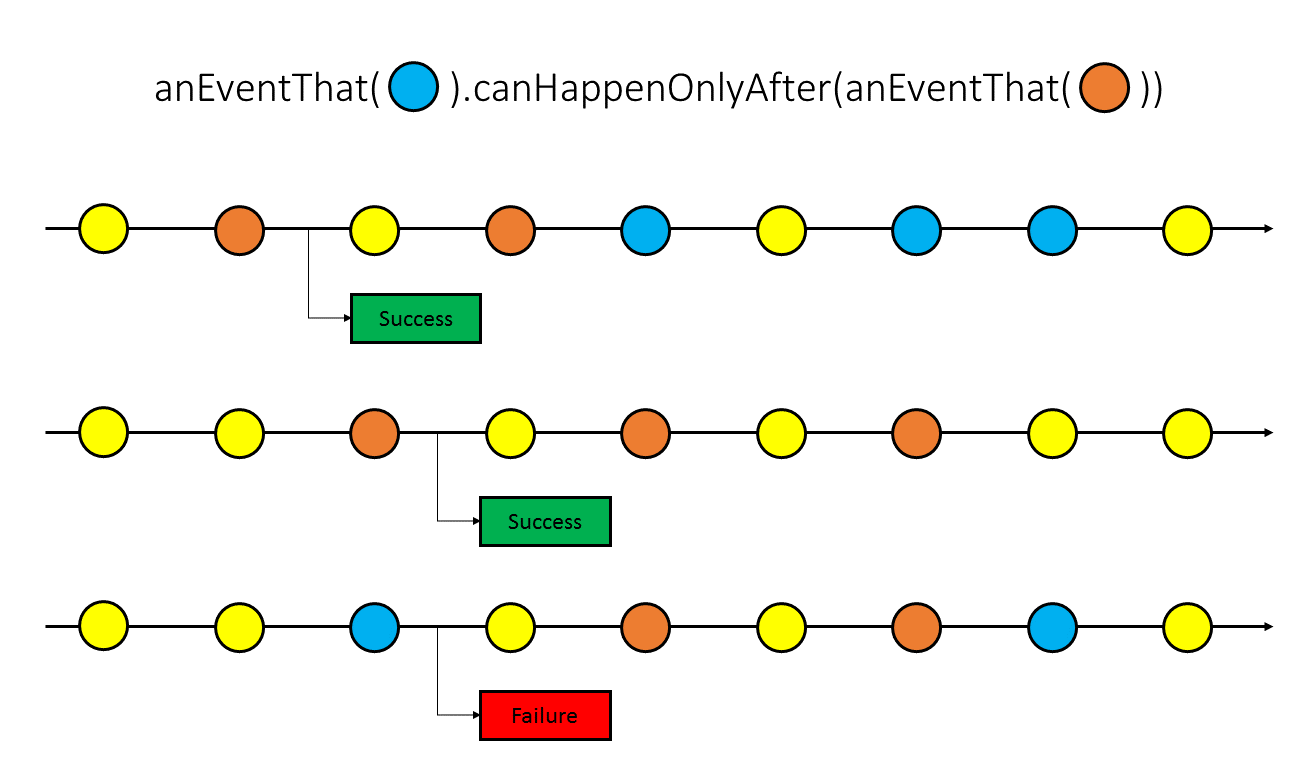
\includegraphics[width=400px]{Images/Event/Lang/Slide1.PNG}}
	
	Note in particular that in the second case the checks succeeds even if no blue event occurs: we are  just saying that blue events \textit{can} happen after an orange one.
	
  	\\ \hline
  	
  \rotatebox[origin=c]{90}{\textbf{ Code Example }} & 
  
  	\begin{lstlisting}
	/* Check race condition with maps */
	anEventThat(isMarkerPlacement())
		.canHappenOnlyAfter(anEventThat(isMapReady()))
	\end{lstlisting}
	
  	\\ \hline  	
  	 
\end{longtable}
\egroup
\end{center}

\subsubsection{Can Happen Only Before}

\begin{center}
\bgroup
\def\arraystretch{1.5}%
\begin{longtable}{ | m{0.3cm} | m{15cm} | }
  \hline
  
  \rotatebox[origin=c]{90}{\textbf{ Structure }} & 
  
  	\begin{lstlisting}
	anEventThat(m1).canHappenOnlyBefore(anEventThat(m2))
	\end{lstlisting}
	
  	\\ \hline
  	 
  \rotatebox[origin=c]{90}{\textbf{ Description }} & 
  
  	Checks that the events that match \texttt{m1} happen only before any event that matches \texttt{m2}, i.e. there cannot be an event that matches \texttt{m1} after the last event that matches \texttt{m2}.
	
  	\\ \hline

  \rotatebox[origin=c]{90}{\textbf{ FOL }} & 
  
  	\begin{multline*}
	\forall e1 \bigg( match(e1, m1) \Rightarrow \exists e2 \Big( match(e2, m2) \land before(e1, e2) \Big) \bigg)
	\end{multline*}
	
  	\\ \hline

  \rotatebox[origin=c]{90}{\textbf{ Visual }} & 
  
	\raisebox{-230pt}{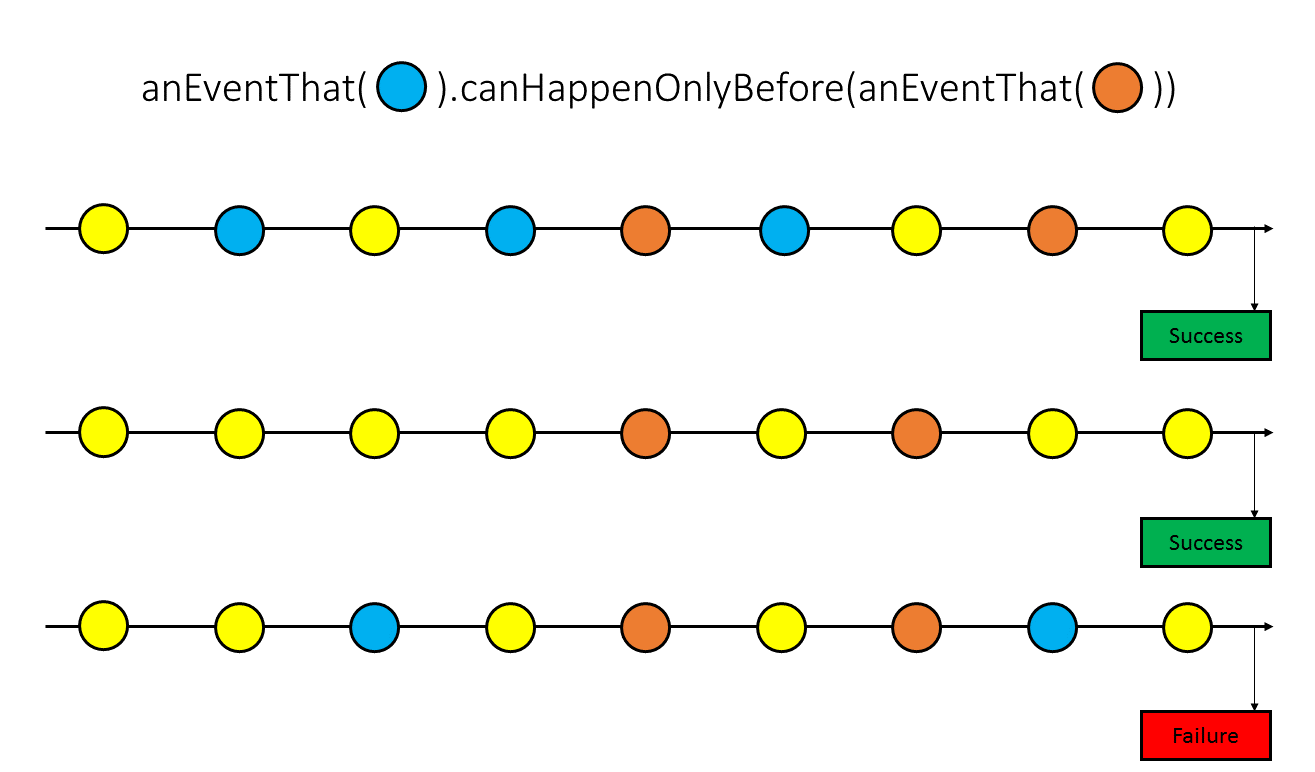
\includegraphics[width=400px]{Images/Event/Lang/Slide2.PNG}}
	
	
  	\\ \hline
  	
  \rotatebox[origin=c]{90}{\textbf{ Code Example }} & 
  
  	\begin{lstlisting}
	/* Can change form input only before it is submitted */
	anEventThat(isTextChangeFrom(usernameTextView))
		.canHappenOnlyBefore(anEventThat(isSubmitForm()))
	\end{lstlisting}
	
  	\\ \hline  	
  	 
\end{longtable}
\egroup
\end{center}

\subsubsection{Can Happen Only Between}

\begin{center}
\bgroup
\def\arraystretch{1.5}%
\begin{longtable}{ | m{0.3cm} | m{15cm} | }
  \hline
  
  \rotatebox[origin=c]{90}{\textbf{ Structure }} & 
  
  	\begin{lstlisting}
	anEventThat(m1).canHappenOnlyBetween(anEventThat(m2), anEventThat(m3))
	\end{lstlisting}
	
  	\\ \hline
  	 
  \rotatebox[origin=c]{90}{\textbf{ Description }} & 
  
  	Checks that the events that match \texttt{m1} happen only between any pair of events that match \texttt{m2} and \texttt{m3} respectively, i.e. there cannot be an event that matches \texttt{m1} before the first event that matches \texttt{m2} or after the last event that matches \texttt{m3}. 
	
  	\\ \hline

  \rotatebox[origin=c]{90}{\textbf{ FOL }} & 
  
  	\begin{multline*}
	\forall e1 \bigg( match(e1, m1) \Rightarrow \exists e2, e3 \Big( match(e2, m2) \land match(e3, m3) \\ \land between(e2, e1, e3) \Big) \bigg)
	\end{multline*}
	
  	\\ \hline

  \rotatebox[origin=c]{90}{\textbf{ Visual }} & 
  
	\raisebox{-230pt}{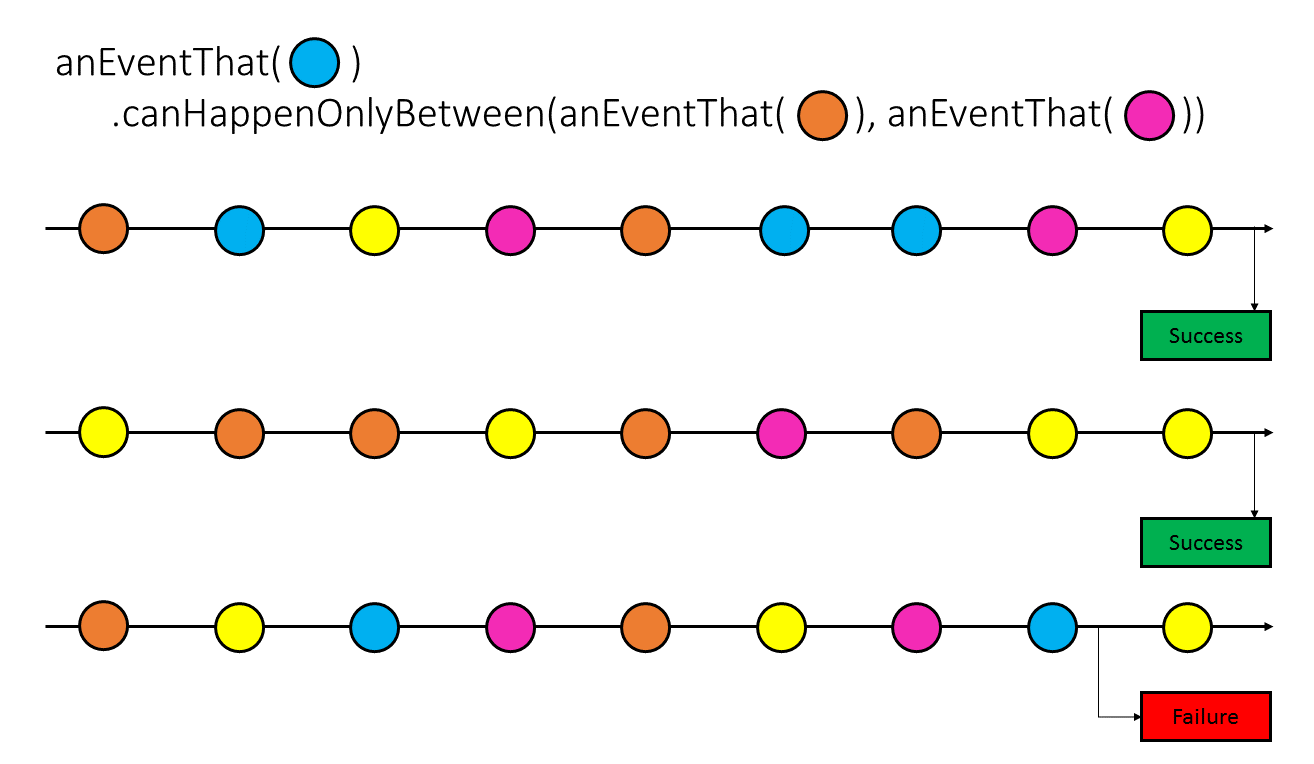
\includegraphics[width=400px]{Images/Event/Lang/Slide3.PNG}}
	
	
  	\\ \hline
  	
  \rotatebox[origin=c]{90}{\textbf{ Code Example }} & 
  
  	\begin{lstlisting}
	/* Can send broadcast only if the the service is working */
	anEventThat(isSendBroadcast())
		.canHappenOnlyBetween(
			anEventThat(isServiceStart(mainService)),
			anEventThat(isServiceStop(mainService)))
	\end{lstlisting}
	
  	\\ \hline  	
  	 
\end{longtable}
\egroup
\end{center}

\subsection{Checks on Sets of Events}

These checks work on sets of events: for example we may say that a certain event generates a set of \textit{n} other events. The cardinality of each set is specified by the quantifiers:
\begin{itemize}
	\item Exactly
	\item At most
	\item At least
\end{itemize}
Only the formulas for "exactly" will be written since the others can be derived by analogy.\bigskip \\
First Order Logic specifications use the counting quantifiers~\cite{Pratt-Hartmann:2014:LCE:2603088.2603117} as a notational shorthand, i.e. $\exists_{=n} x$ means that there exist exactly \textit{n} elements \textit{x}.

\subsubsection{Must Happen After}

\begin{center}
\bgroup
\def\arraystretch{1.5}%
\begin{longtable}{ | m{0.3cm} | m{15cm} | }
  \hline
  
  \rotatebox[origin=c]{90}{\textbf{ Structure }} & 
  
  	\begin{lstlisting}
	exactly(n).eventsWhereEach(m1).mustHappenAfter(anEventThat(m2))
	\end{lstlisting}
	
  	\\ \hline
  	 
  \rotatebox[origin=c]{90}{\textbf{ Description }} & 
  
  	Checks that exactly \texttt{n} events that match \texttt{m1} happen exclusively after every event that matches \texttt{m2}. "Exclusively" means that there cannot be another event that matches \texttt{m2} before the sequence of \texttt{n} events is completed.
	
  	\\ \hline

  \rotatebox[origin=c]{90}{\textbf{ FOL }} & 
  
  	\begin{multline*}
	\forall e2 \Bigg( match(e2, m2) \Rightarrow \exists_{=n} e1 \bigg( match(e1, m1) \land before(e2, e1) \\ \land \neg \exists e2' \Big( match(e2', m2) \land between(e2, e2', e1) \Big) \bigg) \Bigg)
	\end{multline*}
	
  	\\ \hline

  \rotatebox[origin=c]{90}{\textbf{ Visual }} & 
  
	\raisebox{-280pt}{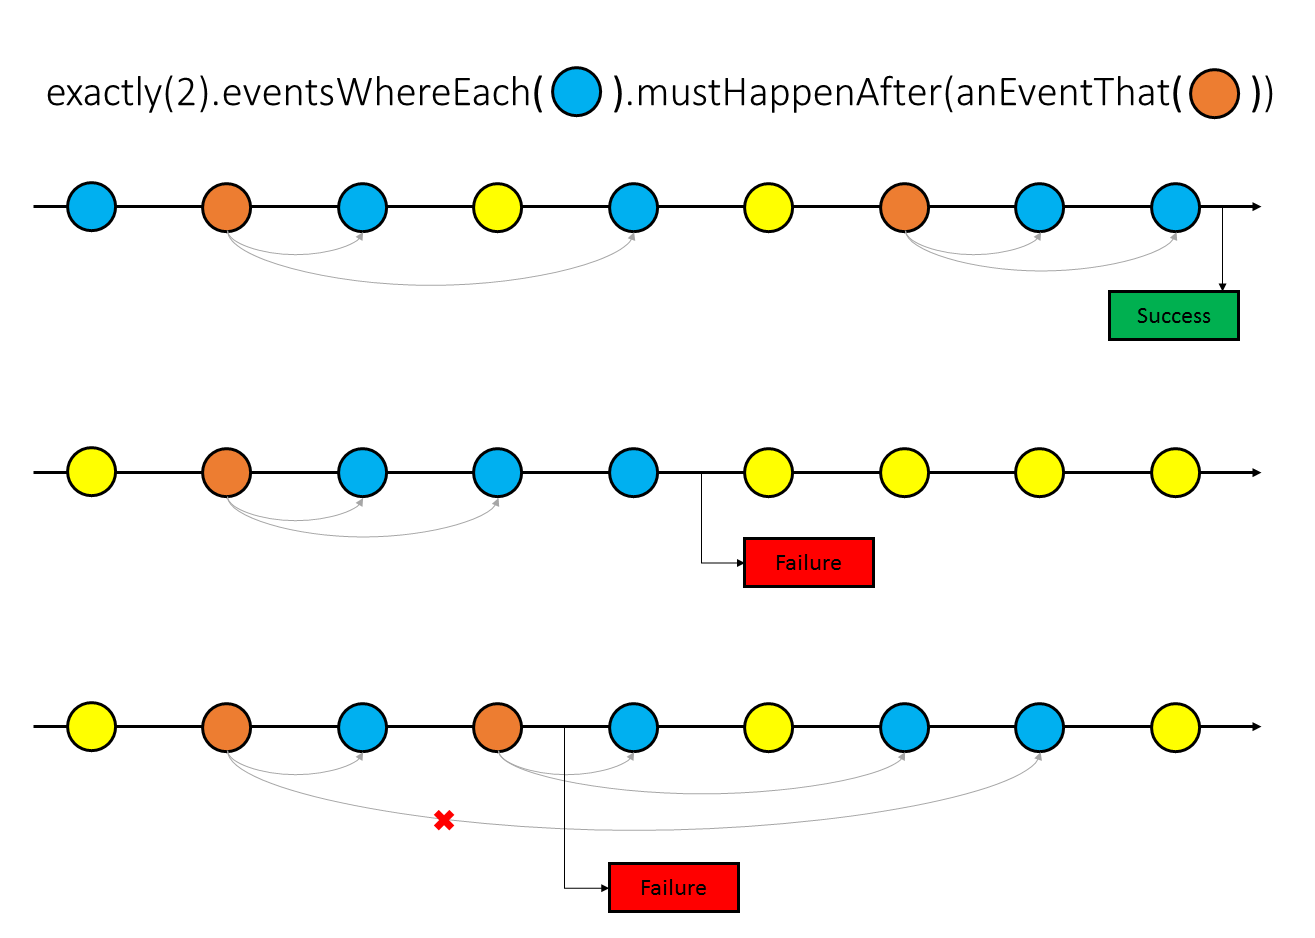
\includegraphics[width=400px]{Images/Event/Lang/Slide4.PNG}}
	
	Note in particular that the third case shows the "exclusively" constraint mentioned before: the check fails because we do not have two blue events after the first orange but before the second one (i.e. the first orange event does \textit{not} match one of the three blue events that follow the second orange event)

  	\\ \hline
  	
  \rotatebox[origin=c]{90}{\textbf{ Code Example }} & 
  
  	\begin{lstlisting}
	/* If a location change happens, the text view must be updated exactly once */	
	exactly(1).eventsWhereEach(isTextChangeFrom(locationTextView))
		.mustHappenAfter(anEventThat(isLocationChange()))
	\end{lstlisting}
	
  	\\ \hline  	
  	 
\end{longtable}
\egroup
\end{center}

\subsubsection{Must Happen Before}

\begin{center}
\bgroup
\def\arraystretch{1.5}%
\begin{longtable}{ | m{0.3cm} | m{15cm} | }
  \hline
  
  \rotatebox[origin=c]{90}{\textbf{ Structure }} & 
  
  	\begin{lstlisting}
	exactly(n).eventsWhereEach(m1).mustHappenBefore(anEventThat(m2))
	\end{lstlisting}
	
  	\\ \hline
  	 
  \rotatebox[origin=c]{90}{\textbf{ Description }} & 
  
  	Checks that exactly \texttt{n} events that match \texttt{m1} happen exclusively before every event that matches \texttt{m2}. "Exclusively" means that the sequence of \texttt{n} events must be after the previous (if any) event that matches \texttt{m2}.
	
  	\\ \hline

  \rotatebox[origin=c]{90}{\textbf{ FOL }} & 
  
  	\begin{multline*}
	\forall e2 \Bigg( match(e2, m2) \Rightarrow \exists_{=n} e1 \bigg( match(e1, m1) \land before(e1, e2) \\ \land \neg \exists e2' \Big( match(e2', m2) \land between(e1, e2', e2) \Big) \bigg) \Bigg)
	\end{multline*}
	
  	\\ \hline

  \rotatebox[origin=c]{90}{\textbf{ Visual }} & 
  
	\raisebox{-280pt}{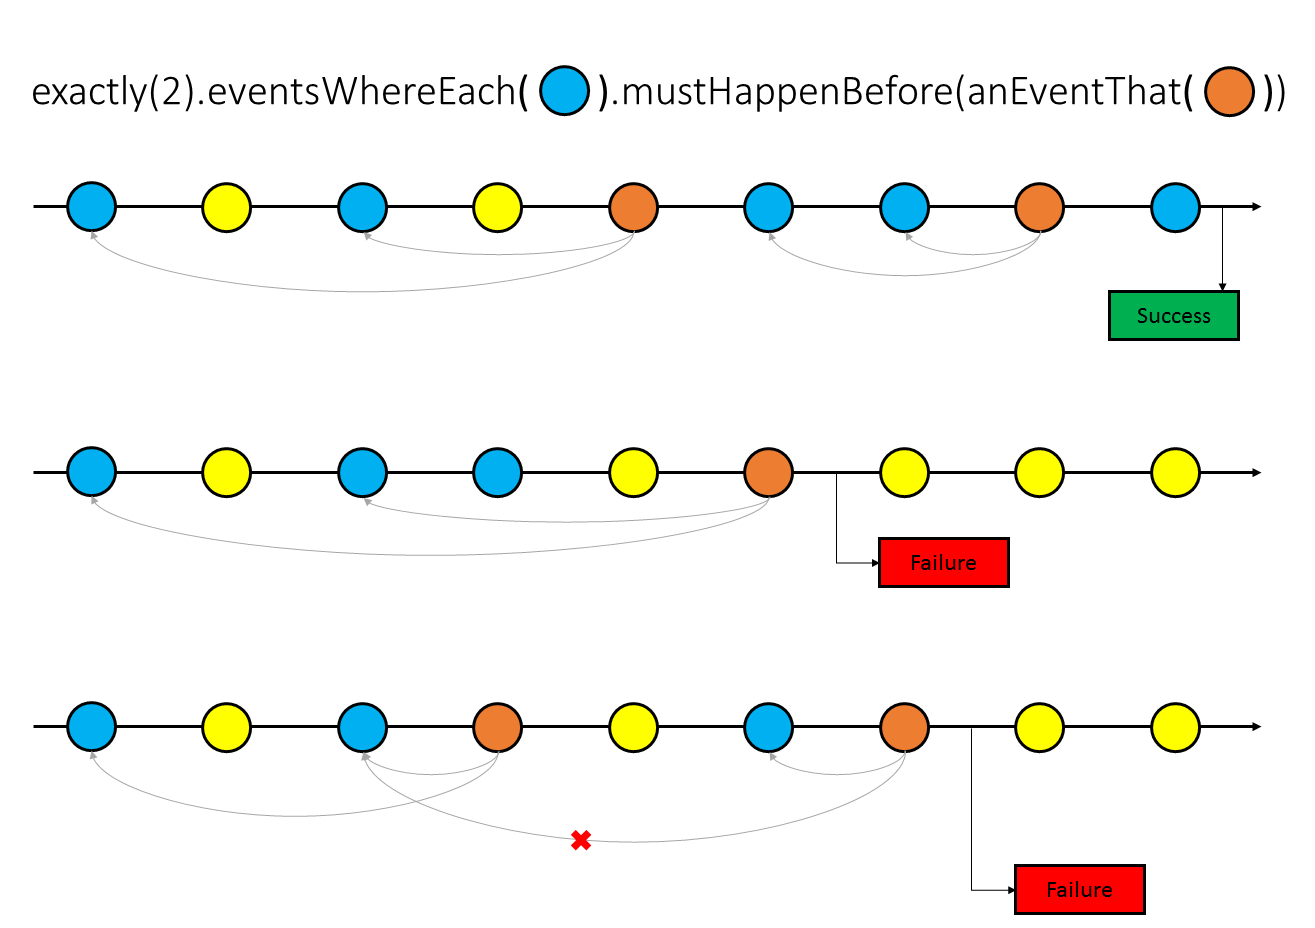
\includegraphics[width=400px]{Images/Event/Lang/Slide5.PNG}}
	
	
  	\\ \hline
  	
  \rotatebox[origin=c]{90}{\textbf{ Code Example }} & 
  
  	\begin{lstlisting}
	/* To setup the list of data the system must perform exactly 3 database queries */
	exactly(3).eventsWhereEach(isDatabaseQuery())
		.mustHappenBefore(anEventThat(isListSetup()))
	\end{lstlisting}
	
  	\\ \hline  	
  	 
\end{longtable}
\egroup
\end{center}

\subsubsection{Must Happen Between}

\begin{center}
\bgroup
\def\arraystretch{1.5}%
\begin{longtable}{ | m{0.3cm} | m{15cm} | }
  \hline
  
  \rotatebox[origin=c]{90}{\textbf{ Structure }} & 
  
  	\begin{lstlisting}
	exactly(n).eventsWhereEach(m1).mustHappenBetween(AnEventThat(m2), AnEventThat(m3))
	\end{lstlisting}
	
  	\\ \hline
  	 
  \rotatebox[origin=c]{90}{\textbf{ Description }} & 
  
  	Checks that exactly \texttt{n} events that match \texttt{m1} happen between every pair of events that match \texttt{m2} and \texttt{m3} respectively.
	
  	\\ \hline

  \rotatebox[origin=c]{90}{\textbf{ FOL }} & 
  
  	\begin{multline*}
	\forall e2 \Bigg( match(e2, m2) \Rightarrow \exists e3 \bigg( \Big( match(e3, m3) \land before(e2, e3) \\ \land \neg \exists e2', e3' \big( match(e2', m2) \land between(e2, e2', e3) \lor match(e3', m3) \\ \land between(e2, e3', e3) \big) \Big) \iff \exists_{=n} e1 \Big( match(e1, m1) \land between(e2, e1, e3 \Big) \bigg) \Bigg)
	\end{multline*}
	
  	\\ \hline

  \rotatebox[origin=c]{90}{\textbf{ Visual }} & 
  
	\raisebox{-190pt}{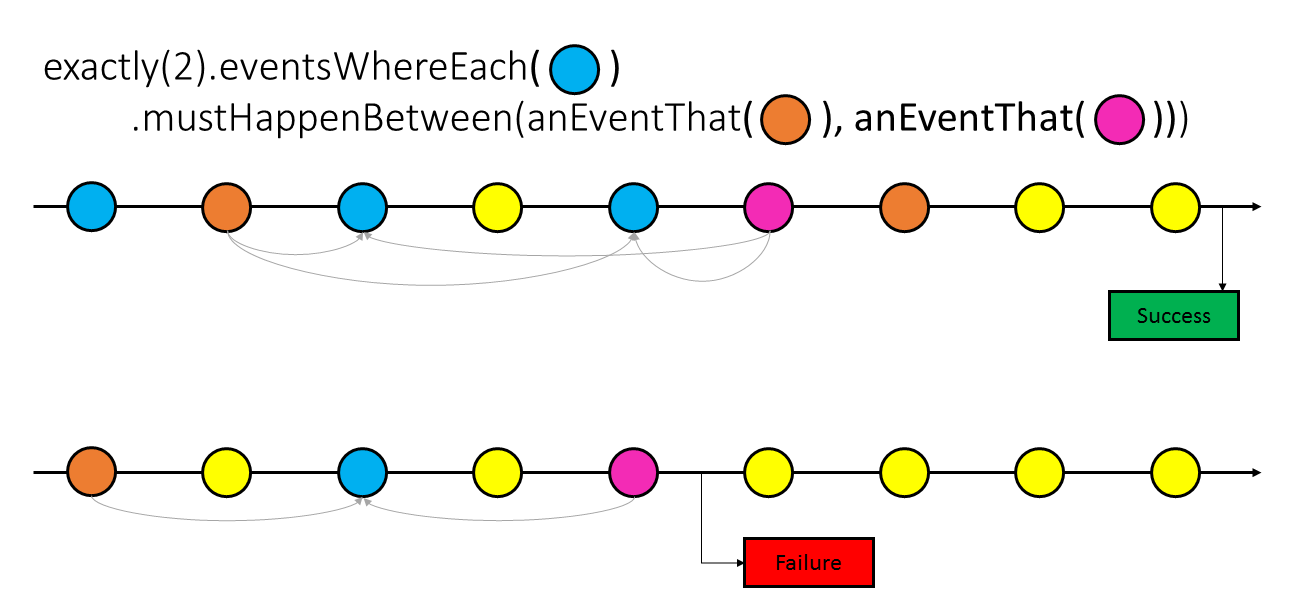
\includegraphics[width=400px]{Images/Event/Lang/Slide6.PNG}}
	
	
  	\\ \hline
  	
  \rotatebox[origin=c]{90}{\textbf{ Code Example }} & 
  
  	\begin{lstlisting}
	/* During the execution of the activity the text is changed exactly four times */
	exactly(4).eventsWhereEach(isTextChangeFrom(myTextView))
		.mustHappenBetween(
			anEventThat(isActivityLifecycleEvent("onResume")),
			anEventThat(isActivityLifecycleEvent("onPause")))
	\end{lstlisting}
	
  	\\ \hline  	
  	 
\end{longtable}
\egroup
\end{center}


\subsection{Checks on the Whole Stream}

The third type of checks concerns the entire stream of events: they allow for example to specify the number of all the events of a certain type in the whole sequence generated by a particular execution.

\subsubsection{Match In Order}

\begin{center}
\bgroup
\def\arraystretch{1.5}%
\begin{longtable}{ | m{0.3cm} | m{15cm} | }
  \hline
  
  \rotatebox[origin=c]{90}{\textbf{ Structure }} & 
  
  	\begin{lstlisting}[mathescape]
	allEventsWhereEach(m).matchInOrder(m$_1$, m$_2$, ... , m$_n$)
	\end{lstlisting}
	
  	\\ \hline
  	 
  \rotatebox[origin=c]{90}{\textbf{ Description }} & 
  
  	Checks that \textit{all} the events that match \texttt{m} match in order the given matchers.
	
  	\\ \hline

  \rotatebox[origin=c]{90}{\textbf{ FOL }} & 
  
  	\begin{multline*}
	\forall e \bigg( match(e, m) \Rightarrow \exists i \Big( indexOf(e, m, i) \land match(e, m_i) \Big) \bigg)\\\\
indexOf(e, m, i) \equiv \exists_{=i} e' \Big( match(e', m) \land before(e', e) \Big)
	\end{multline*}
	
  	\\ \hline

  \rotatebox[origin=c]{90}{\textbf{ Visual }} & 
  
	\raisebox{-230pt}{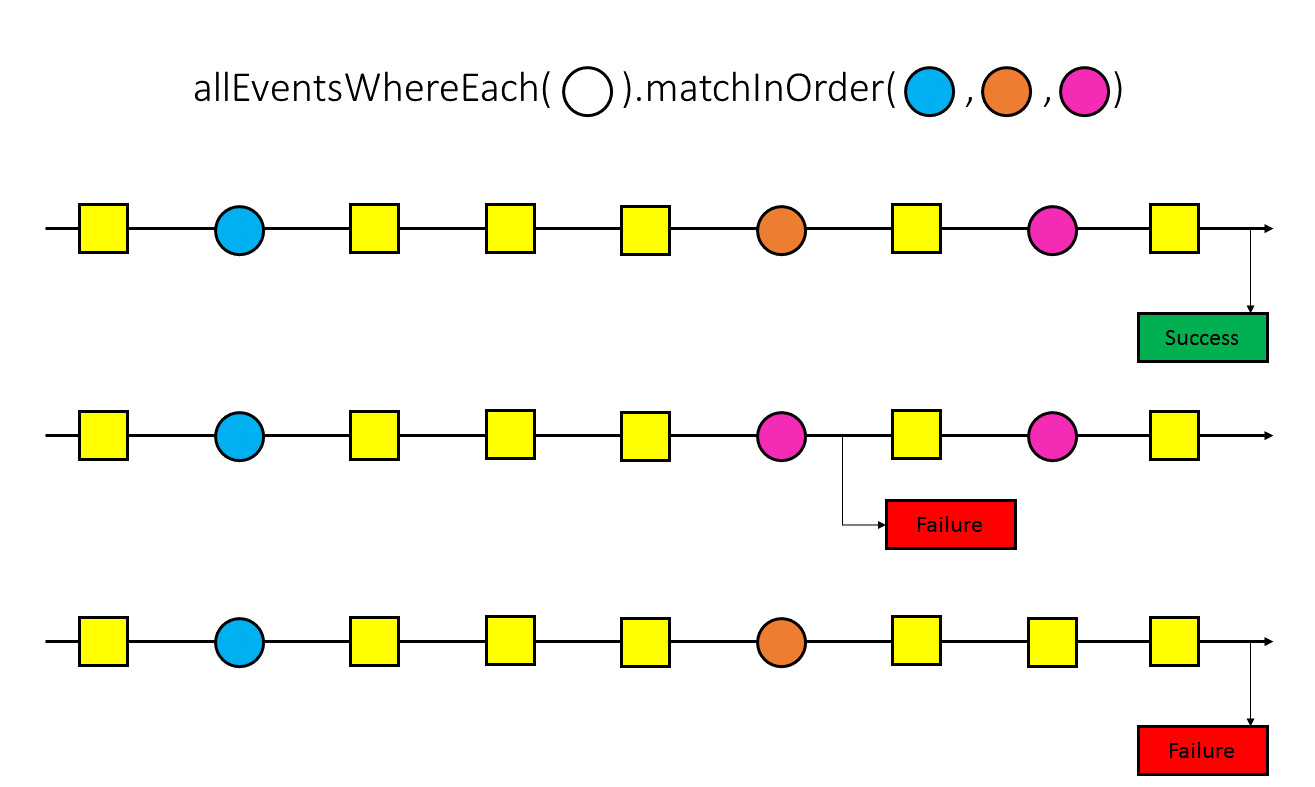
\includegraphics[width=400px]{Images/Event/Lang/Slide7.PNG}}
	
	Note in particular the last case: the check implicitly states that the events must be exactly 3 and they must satisfy the three matchers.	If the third one is missing, the check fails.
	
  	\\ \hline
  	
  \rotatebox[origin=c]{90}{\textbf{ Code Example }} & 
  
  	\begin{lstlisting}
	/* Defines the only valid fragment backstack changes sequence */	
	allEventsWhereEach(isFragmentBackstackChange())
		.matchInOrder(
			isFragmentBackstackPush(mainFragment),
			isFragmentBackstackPush(languageFragment),
			isFragmentBackstackPush(gameFragment),
			isFragmentBackstackPop(mainFragment))
	\end{lstlisting}
	
  	\\ \hline  	
  	 
\end{longtable}
\egroup
\end{center}

\subsubsection{Are Ordered}

\begin{center}
\bgroup
\def\arraystretch{1.5}%
\begin{longtable}{ | m{0.3cm} | m{15cm} | }
  \hline
  
  \rotatebox[origin=c]{90}{\textbf{ Structure }} & 
  
  	\begin{lstlisting}
	allEventsWhereEach(m).areOrdered(f)
	\end{lstlisting}
	
  	\\ \hline
  	 
  \rotatebox[origin=c]{90}{\textbf{ Description }} & 
  
  	Checks that \textit{all} the events that match \texttt{m} are in the order defined by the comparator function \textit{f} (receives two events and returns an integer $<$ 0 if the first is less than the second, 0 if they are equal, and $>$ 0 if the first is greater than the second).
	
  	\\ \hline

  \rotatebox[origin=c]{90}{\textbf{ FOL }} & 
  
  	\begin{multline*}
	\forall e, e' \bigg( match(e, m) \land match(e', m) \land before(e, e') \land\\ \neg \exists e'' \Big( match(e'', m) \land between(e, e'', e') \Big) \Rightarrow ordered(f, e, e') \bigg)\\\\
ordered(com, e1, e2) \equiv \bigg( \Big( com<0 \Rightarrow before(e1, e2) \Big) \lor\\ \Big( com=0 \Rightarrow before(e1, e2) \lor before(e2, e1) \Big) \lor\\ \Big( com>0 \Rightarrow before(e2, e1) \Big) \bigg)
	\end{multline*}
	
  	\\ \hline

  \rotatebox[origin=c]{90}{\textbf{ Visual }} & 
  
	\raisebox{-160pt}{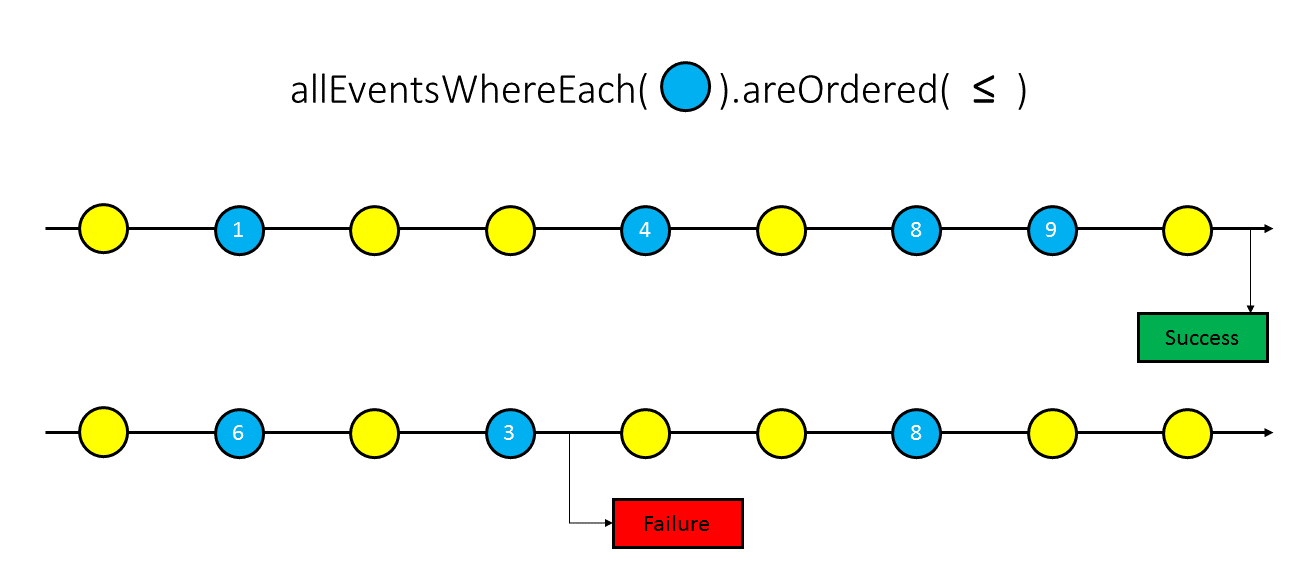
\includegraphics[width=400px]{Images/Event/Lang/Slide8.PNG}}
	
	
  	\\ \hline
  	
  \rotatebox[origin=c]{90}{\textbf{ Code Example }} & 
  
  	\begin{lstlisting}
	/* The text in the countdown is updated in the correct (inverse) order */
	allEventsWhereEach(isTextChangeFrom(countdownView))
		.areOrdered(new Comparator<Event>()
					{
						@Override
						public int compare(Event lhs, Event rhs)
						{
							String t1 = ((TextChangeEvent) lhs).getText();
							String t2 = ((TextChangeEvent) rhs).getText();
							return Integer.compare(Integer.valueOf(t2), Integer.valueOf(t1));
						}
					}));
	\end{lstlisting}
	
  	\\ \hline  	
  	 
\end{longtable}
\egroup
\end{center}

\subsubsection{Exists An Event}

\begin{center}
\bgroup
\def\arraystretch{1.5}%
\begin{longtable}{ | m{0.3cm} | m{15cm} | }
  \hline
  
  \rotatebox[origin=c]{90}{\textbf{ Structure }} & 
  
  	\begin{lstlisting}
	existsAnEventThat(m)
	\end{lstlisting}
	
  	\\ \hline
  	 
  \rotatebox[origin=c]{90}{\textbf{ Description }} & 
  
  	Checks that at least one event that matches the matcher \texttt{m} exists anywhere in the sequence.
	
  	\\ \hline

  \rotatebox[origin=c]{90}{\textbf{ FOL }} & 
  
  	\begin{multline*}
	\exists e \Big( match(e, m) \Big)
	\end{multline*}
	
  	\\ \hline

  \rotatebox[origin=c]{90}{\textbf{ Visual }} & 
  
	\raisebox{-170pt}{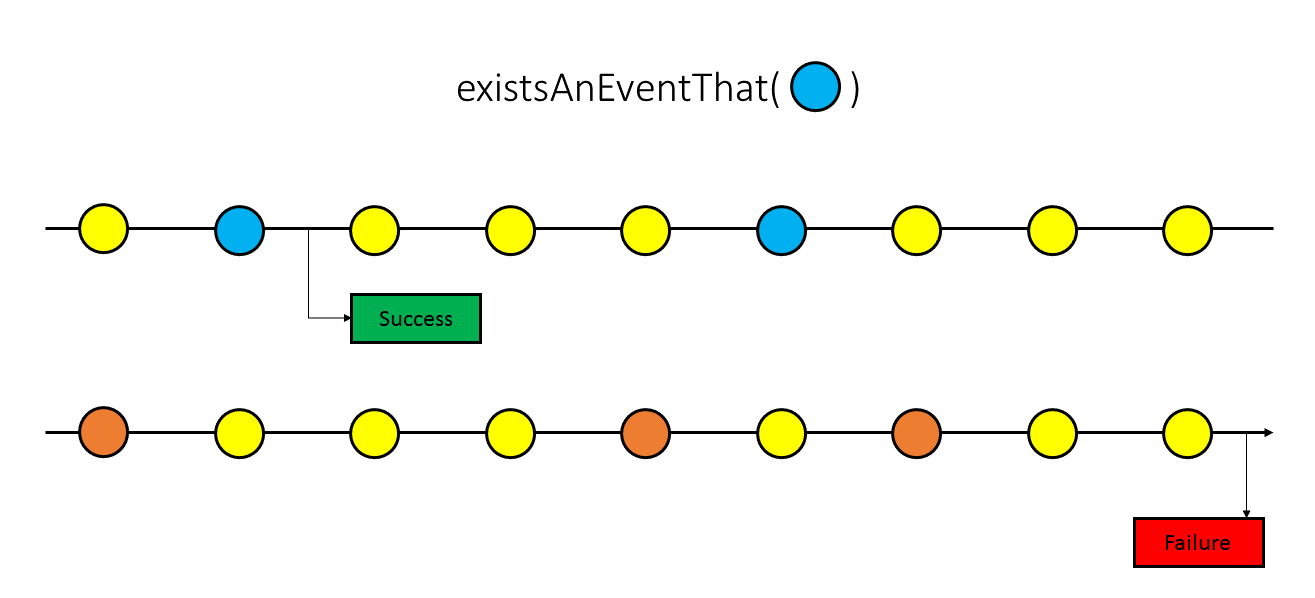
\includegraphics[width=400px]{Images/Event/Lang/Slide9.PNG}}
	
	
  	\\ \hline
  	
  \rotatebox[origin=c]{90}{\textbf{ Code Example }} & 
  
  	\begin{lstlisting}
	/* The database must be opened sooner or later during the execution */
	existsAnEventThat(isOpenDatabase())
	\end{lstlisting}
	
  	\\ \hline  	
  	 
\end{longtable}
\egroup
\end{center}

\subsubsection{Exist Events}

\begin{center}
\bgroup
\def\arraystretch{1.5}%
\begin{longtable}{ | m{0.3cm} | m{15cm} | }
  \hline
  
  \rotatebox[origin=c]{90}{\textbf{ Structure }} & 
  
  	\begin{lstlisting}
	exist(exactly(n)).eventsWhereEach(m)
	\end{lstlisting}
	
  	\\ \hline
  	 
  \rotatebox[origin=c]{90}{\textbf{ Description }} & 
  
  	Checks that \textit{all} the events that match \texttt{m} are exactly \texttt{n}.
	
  	\\ \hline

  \rotatebox[origin=c]{90}{\textbf{ FOL }} & 
  
  	\begin{multline*}
	\exists_{=n} e \Big( match(e, m) \Big)
	\end{multline*}
	
  	\\ \hline

  \rotatebox[origin=c]{90}{\textbf{ Visual }} & 
  
	\raisebox{-170pt}{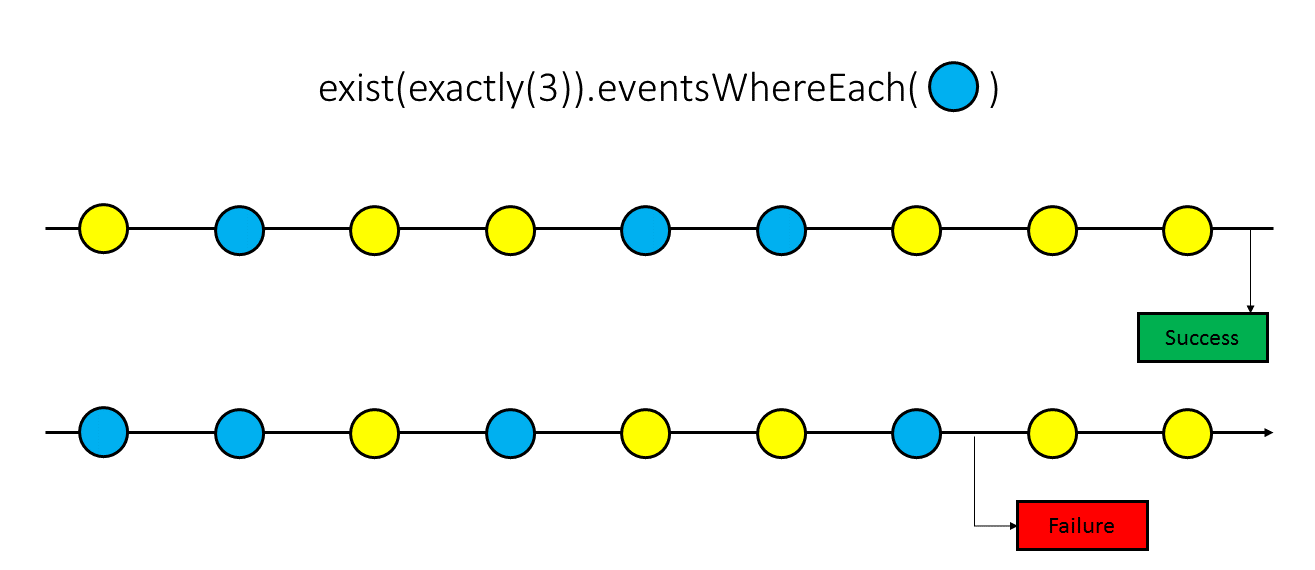
\includegraphics[width=400px]{Images/Event/Lang/Slide10.PNG}}
	
	
  	\\ \hline
  	
  \rotatebox[origin=c]{90}{\textbf{ Code Example }} & 
  
  	\begin{lstlisting}
	/* In this execution the system sends exactly 10 broadcasts */
	exist(exactly(10))
		.eventsWhereEach(isSendBroadcast())
	\end{lstlisting}
	
  	\\ \hline  	
  	 
\end{longtable}
\egroup
\end{center}

In the same way seen in the previous section, the checks for "at most" and "at least" can be derived by analogy.

\subsection{Connectives between Checks}

These constructs allow to specify the standard logic connectives between one or more of the previously defined consistency checks.

\subsubsection{And}

\begin{center}
\bgroup
\def\arraystretch{1.5}%
\begin{longtable}{ | m{0.3cm} | m{15cm} | }
  \hline
  
  \rotatebox[origin=c]{90}{\textbf{ Structure }} & 
  
  	\begin{lstlisting}
	allHold(c1, c2,...)
	\end{lstlisting}
	
  	\\ \hline
  	 
  \rotatebox[origin=c]{90}{\textbf{ Description }} & 
  
  	All sub-checks \textit{c1}, \textit{c2}, etc. must succeed.
	
  	\\ \hline

  \rotatebox[origin=c]{90}{\textbf{ FOL }} & 
  
  	\begin{multline*}
	c1 \land c2 \land ...
	\end{multline*}
	
  	\\ \hline

  \rotatebox[origin=c]{90}{\textbf{ Visual }} & 
  
	\raisebox{-105pt}{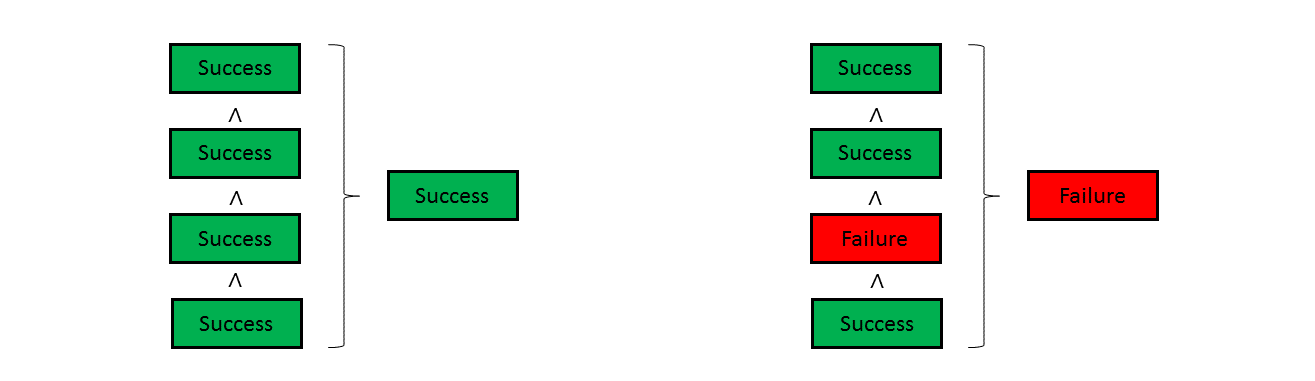
\includegraphics[width=400px]{Images/Event/Lang/Slide11.png}}
	
	
  	\\ \hline
  	
  \rotatebox[origin=c]{90}{\textbf{ Code Example }} & 
  
  	\begin{lstlisting}
	/* The service must only be started after the button is clicked */
	allHold(
		anEventThat(isStartService())
			.canHappenOnlyAfter(isClickOn(startButton)),
		exactly(1).eventsWhereEach(isStartService())
			.mustHappenAfter(isClickOn(startButton)))
	\end{lstlisting}
	
  	\\ \hline  	
  	 
\end{longtable}
\egroup
\end{center}

\subsubsection{Or}

\begin{center}
\bgroup
\def\arraystretch{1.5}%
\begin{longtable}{ | m{0.3cm} | m{15cm} | }
  \hline
  
  \rotatebox[origin=c]{90}{\textbf{ Structure }} & 
  
  	\begin{lstlisting}
	anyHolds(c1, c2,...)
	\end{lstlisting}
	
  	\\ \hline
  	 
  \rotatebox[origin=c]{90}{\textbf{ Description }} & 
  
  	At least one sub-check must succeed.
	
  	\\ \hline

  \rotatebox[origin=c]{90}{\textbf{ FOL }} & 
  
  	\begin{multline*}
	c1 \lor c2 \lor ...
	\end{multline*}
	
  	\\ \hline

  \rotatebox[origin=c]{90}{\textbf{ Visual }} & 
  
	\raisebox{-105pt}{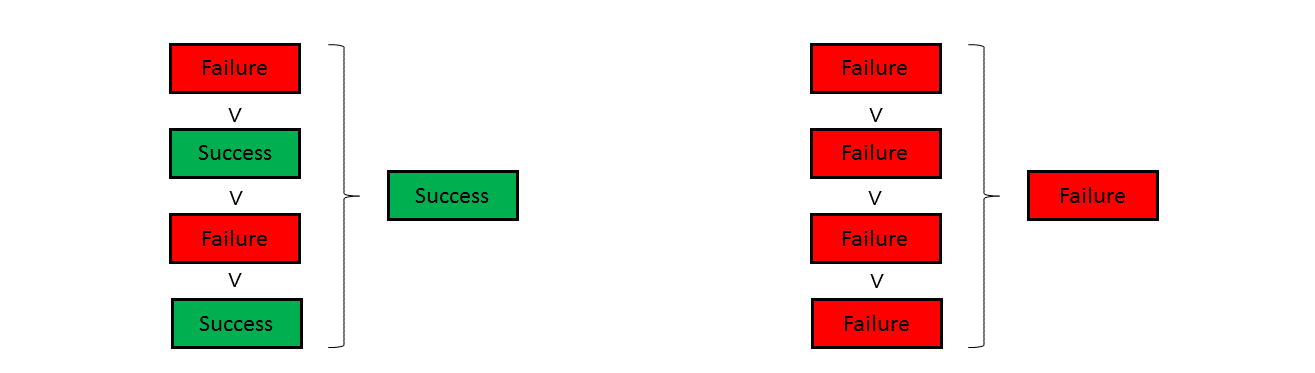
\includegraphics[width=400px]{Images/Event/Lang/Slide12.PNG}}
	
	
  	\\ \hline
  	
  \rotatebox[origin=c]{90}{\textbf{ Code Example }} & 
  
  	\begin{lstlisting}
	/* Either succeed or fail download (no situations where the user is not notified) */		
	anyHolds(
		exist(exactly(1))
			.eventsWhereEach(isDownloadSuccess()),
		exist(exactly(1))
			.eventsWhereEach(isDownloadError()));
	\end{lstlisting}
	
  	\\ \hline  	
  	 
\end{longtable}
\egroup
\end{center}

\subsubsection{Not}

\begin{center}
\bgroup
\def\arraystretch{1.5}%
\begin{longtable}{ | m{0.3cm} | m{15cm} | }
  \hline
  
  \rotatebox[origin=c]{90}{\textbf{ Structure }} & 
  
  	\begin{lstlisting}
	isNotSatisfied(c)
	\end{lstlisting}
	
  	\\ \hline
  	 
  \rotatebox[origin=c]{90}{\textbf{ Description }} & 
  
  	Inverts the outcome of the sub-check.
	
  	\\ \hline

  \rotatebox[origin=c]{90}{\textbf{ FOL }} & 
  
  	\begin{multline*}
	\neg c
	\end{multline*}
	
  	\\ \hline

  \rotatebox[origin=c]{90}{\textbf{ Visual }} & 
  
	\raisebox{-70pt}{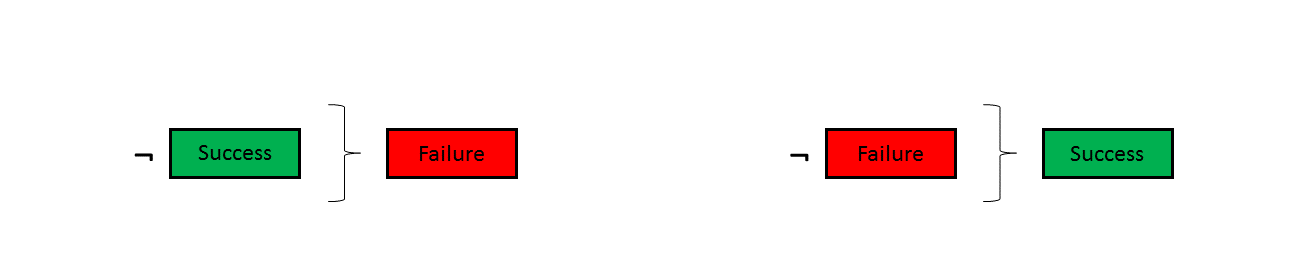
\includegraphics[width=400px]{Images/Event/Lang/Slide13.PNG}}
	
	
  	\\ \hline
  	
  \rotatebox[origin=c]{90}{\textbf{ Code Example }} & 
  
  	\begin{lstlisting}
	/* In this execution the email draft cannot be saved */		
	isNotSatisfied(
		existsAnEventThat(isSaveDraft()))
	\end{lstlisting}
	
  	\\ \hline  	
  	 
\end{longtable}
\egroup
\end{center}

\subsubsection{Single Implication}

\begin{center}
\bgroup
\def\arraystretch{1.5}%
\begin{longtable}{ | m{0.3cm} | m{15cm} | }
  \hline
  
  \rotatebox[origin=c]{90}{\textbf{ Structure }} & 
  
  	\begin{lstlisting}
	providedThat(c1).then(c2)
	\end{lstlisting}
	
  	\\ \hline
  	 
  \rotatebox[origin=c]{90}{\textbf{ Description }} & 
  
  	\texttt{c2} is checked only if \texttt{c1} succeeds.
	
  	\\ \hline

  \rotatebox[origin=c]{90}{\textbf{ FOL }} & 
  
  	\begin{multline*}
	c1 \Rightarrow c2
	\end{multline*}
	
  	\\ \hline

  \rotatebox[origin=c]{90}{\textbf{ Visual }} & 
  
	\raisebox{-140pt}{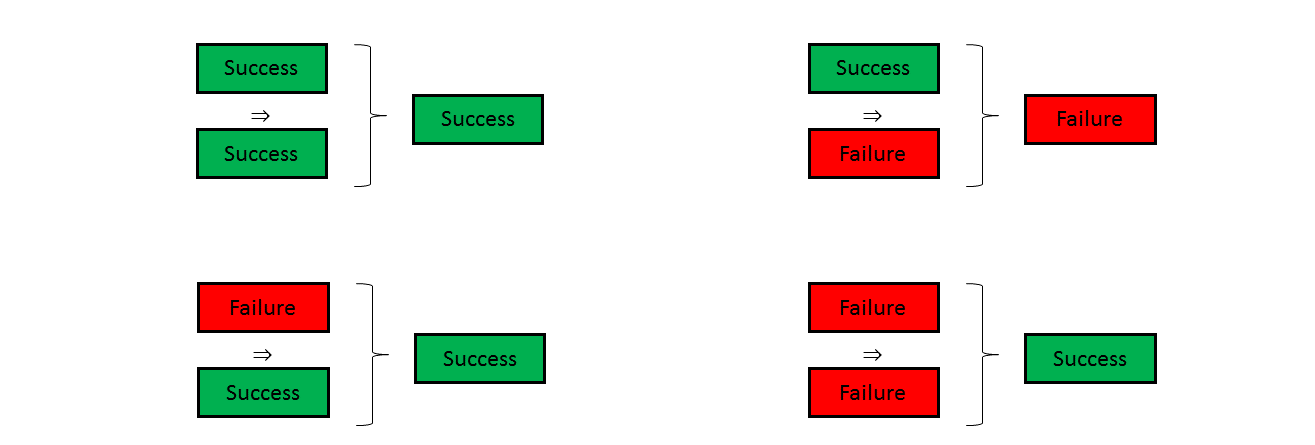
\includegraphics[width=400px]{Images/Event/Lang/Slide14.PNG}}
	
	
  	\\ \hline
  	
  \rotatebox[origin=c]{90}{\textbf{ Code Example }} & 
  
  	\begin{lstlisting}
	/* If the list order changes, then we must update the database */
	providedThat(
			exist(atLeast(1))
				.eventsWhereEach(isListOrderChange()))
		.then(
			exist(exactly(1))
				.eventsWhereEach(isSaveDatabase()))
	\end{lstlisting}
	
  	\\ \hline  	
  	 
\end{longtable}
\egroup
\end{center}

\subsubsection{Double Implication}

\begin{center}
\bgroup
\def\arraystretch{1.5}%
\begin{longtable}{ | m{0.3cm} | m{15cm} | }
  \hline
  
  \rotatebox[origin=c]{90}{\textbf{ Structure }} & 
  
  	\begin{lstlisting}
	isSatisfied(c1).iff(c2)
	\end{lstlisting}
	
  	\\ \hline
  	 
  \rotatebox[origin=c]{90}{\textbf{ Description }} & 
  
  	Succeeds only if both sub-checks fail or both succeed.
	
  	\\ \hline

  \rotatebox[origin=c]{90}{\textbf{ FOL }} & 
  
  	\begin{multline*}
	c1 \iff c2
	\end{multline*}
	
  	\\ \hline

  \rotatebox[origin=c]{90}{\textbf{ Visual }} & 
  
	\raisebox{-140pt}{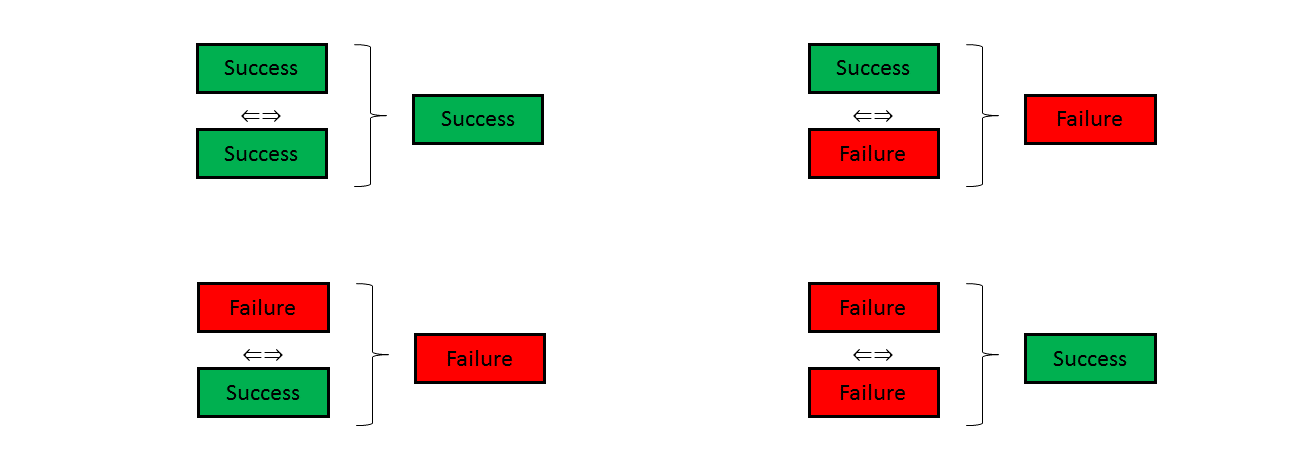
\includegraphics[width=400px]{Images/Event/Lang/Slide15.PNG}}
	
	
  	\\ \hline
  	
  \rotatebox[origin=c]{90}{\textbf{ Code Example }} & 
  
  	\begin{lstlisting}
	/* Send email if and only if the user clicks on the send button */			
	isSatisfied(
			existsAnEventThat(isClickOn(sendButton)))
		.iff(
			existsAnEventThat(isSendEmail()))
	\end{lstlisting}
	
  	\\ \hline  	
  	 
\end{longtable}
\egroup
\end{center}

\section{Design}\label{event_design}
To implement the event-based testing approach described so far, the following main components are employed:
\begin{itemize}
	\item Events: objects that represent events in the application.
	\item Event Generators: structures that actually generate the events whenever something happens in the application.
	\item Checks: ways to specify the consistency rules defined in the previous section.
	\item Results: the outcomes of the checks.
	\item Event Monitor: the main interface of the system, receives the events, applies the checks and produces the results.
\end{itemize}
The following UML class diagram shows an abstract representation of the system:\\
TODO PLACE UML HERE\\
The \textit{EventMonitor} offers methods to add one or more \textit{EventGenerator} objects to define the event stream, to add one or more \textit{Check} objects to be verified and handles the \textit{Result} objects in some way (e.g. makes a test case fail if the \textit{Result} is a failure).\medskip \\
Each \textit{Check} contains the logic of a consistency check: it will receive each \textit{Event} of the stream in order and act accordingly. A \textit{Check} has the possibility to short-circuit its behavior (i.e. interrupt the stream of events if the consistency check succeeds or fails before the end of the sequence). In any case, when it short-circuits or the stream comes to an end, the \textit{Check} produces one and only one \textit{Result} object.\medskip \\
Each \textit{Result} contains an \textit{Outcome} and a message describing it. In particular, an \textit{Outcome} can be a \textit{Success}, a \textit{Failure} and a \textit{Warning}. A \textit{Warning} outcome has not been included in the formal specifications of the checks in the previous section for simplicity: it's meaning is that the \textit{Check} succeeded with some minor error or in a particular situations (for example a check that specifies that an event A always generates exactly one event B may return \textit{Warning} if no event A has been found in the sequence).\medskip \\
A \textit{Descriptor} allows to specify a \textit{Check}. It describes one or more events of the stream and provides some methods to express a condition on those events. In particular, \textit{SingleEvent} describes a single event of a certain type at a time, \textit{SetOfEvents} describes a set of events of a certain type at a time and \textit{AllEvents} describes all the events of a certain type in the whole stream. To determine the type of the events identified by the \textit{Descriptor}, a \textit{Matcher} object is used.\medskip \\
The cardinality of the descriptor \textit{SetOfEvents} is defined by a \textit{Quantifier} that has an integer values as input. A quantifier can be \textit{Exactly}, \textit{AtMost} or \textit{AtLeast}.\medskip \\
Finally, a \textit{CheckConnective} allows to transform one or more \textit{Check} objects into a single \textit{Check}, i.e. it specifies one of the standard logic connectives \textit{Not}, \textit{And}, \textit{Or}, \textit{SingleImplication} and \textit{DoubleImplication}.

\section{Implementation}

For the implementation of event-based testing, the ReactiveX library was chosen. This innovative reactive programming paradigm focuses on data flow: this means generating (statically or dynamically) a flow of events, propagate them and allow interested components to react to them. The idea of reactive programming is fire-and-forget messaging: send a request and asynchronously wait for the response to be ready or, even more importantly, if we are dealing with response sets wait for individual results to be forwarded (without waiting for the whole set to be computed).\bigskip \\
In the next sections a more detailed introduction to the ReactiveX library will be presented, followed by the implementation of the actual event-based testing system.

\subsection{ReactiveX}
The Reactive Extensions (ReactiveX or Rx) are a reactive programming library to compose asynchronous and event-based programs. As defined by its authors, ReactiveX is a combination of the best ideas from:
\begin{itemize}
	\item The Observer pattern (design pattern where a subject automatically notifies the so-called observers of its state changes).
	\item The Iterator pattern (design pattern where an iterator is used to traverse a collection of elements, like an array).
	\item Functional Programming (declarative programming paradigm where computation is performed via mathematical functions that are not allowed to change the state of the system).
\end{itemize}
This approach is asynchronous because many instructions may execute in parallel and their results (events) are later captured, in any order, by the listeners. For this reason, the main idea to perform a computation is not to call methods like in classic sequential programming but to define a mechanism to react to results when they are ready.\bigskip \\
ReactiveX programming paradigm is essentially based on three steps:
\begin{itemize}
	\item Create: the Observable components are used to generate event or data streams.
	\item Transform: Operators allow to modify the event streams (e.g. change each event or filter out some of them) and compose them (e.g. join two streams).
	\item Listen: Subscriber components can listen to event streams and receive their elements one by one, to perform some computation.
\end{itemize}
An Observable is in charge of emitting events: it generates zero, one or more than one events (depending on the specific implementation), and then terminates either by successfully completing or with an error. Observables can be "hot" (emit events even if no Subscriber is listening) or "cold" (emit events only after a Subscriber is registered).\medskip \\
An Observable can be modified by an Operator: most operators can be applied on an event stream generated by an Observable to return a new modified event stream. For example the operator \texttt{map(function)} allows to apply a function to each event in the stream (e.g. a stream of numbers modified by a map with a summing function may become a stream where all the original numbers have been increased by 1). Since the result of an operator is an Observable, operators can be applied in chain (i.e. apply an operator on the result of another operator) to achieve complex modifications.\medskip \\
A Subscriber consumes the events emitted by the Observables (that can either be "original" or the result of one or more Operators). Subscribers allow to react to asynchronous results: for example, an Observer may send a network response whenever it is ready, the Subscriber receives it and shows the information to the user.\bigskip \\
The advantages of the Rx paradigm are:
\begin{itemize}
	\item Cross-Platform: it is available in many programming languages, like RxJava, RxSwift, RxJS, RxPHP, etc.
	\item Can be used for any application, from Front-End (e.g. UI events and API responses) to Back-End (e.g. asynchronicity and concurrency).
	\item Operators usually make computations less verbose and more readable
	\item Error handling: if an error occurs in one of the steps of the computation the exception is automatically intercepted by Rx and forwarded to the user via appropriate callbacks.
	\item Easy concurrency: Rx allows to easily specify in which threads the components should be run, without worrying about implementation details.
	\item Extensible: a developer can define custom Observables, Operators and Subscribers to achieve anything an application may require.
\end{itemize}
The characteristics of ReactiveX make this programming paradigm very suitable for many applications. It is successfully employed in industry: examples of users of Rx are Microsoft, Netflix and GitHub.

\subsection{RxJava and RxAndroid}
RxJava~\cite{RxJava} is the Java implementation of ReactiveX. It is an open source project initially developed by Netflix for server-side concurrency. The main reason for its adoption and development was to avoid Java Futures (results of asynchronous computation) and callbacks because both are expensive when composed, especially if nested.\smallskip \\
In addition to implementing all functionalities of ReactiveX paradigm (Observables, Subscribers, Operators, etc.), RxJava also has the advantages of being:
\begin{itemize}
	\item Lightweight: zero dependencies and single small JAR to contain the whole library.
	\item Polyglot: supports Java 6 or higher and JVM-based languages such as Groovy, Clojure, JRuby, Kotlin and Scala.
	\item Composable: several RxJava Libraries are available to developers to manage common use cases.
\end{itemize} \bigskip
RxAndroid~\cite{RxAndroid} is a RxJava module that provides specific bindings for the Android platform, for example to easily specify the main (UI) thread as the observing thread or, more in general, a custom Looper. RxAndroid can in turn be extended by other modules, some of which are listed in the next section.

\subsection{Events Observable in Android}
Several modules allow Android developers to observe many events inside an application. For example, we can observe:
\begin{itemize}
	\item UI Widgets: RxBinding~\cite{RxBinding} module allows to observe user inputs or changes on UI widgets like TextView (e.g. clicks, text change), app bar menu (e.g. option selected), etc.
	\item Settings: RxPreferences~\cite{RxPreferences} module allows to receive events from the Shared Preferences system (storage provided by Android to store the app settings).
	\item Files: RxFileObserver~\cite{RxFileObserver} fires events for file accesses or changes.
	\item Database: StorIO~\cite{StorIO} allows to manage and observe an SQLite database.
	\item Network: ReactiveNetwork~\cite{ReactiveNetwork} detects network changes (e.g. WiFi or mobile connection).
	\item External API Requests: Retrofit~\cite{Retrofit} offers observables to receive network responses (REST client).
	\item Broadcasts: RxBroadcast~\cite{RxBroadcast} builds an event stream from a Broadcast Receiver results.
	\item Location: ReactiveLocation~\cite{ReactiveLocation} allows to observe location changes.
	\item Sensors: ReactiveSensors~\cite{ReactiveSensors} fires events from hardware sensors.
	\item Permissions: RxPermissions~\cite{RxPermissions} allows to receive events from the permissions manager.
	\item Google Maps: RxGoogleMaps~\cite{RxGoogleMaps} fires events related to Google Maps.
	\item Google Wear: RxWear~\cite{RxWear} allows to observe messages to and from a connected smartwatch.
\end{itemize}\bigskip
The utility module RxLifecycle~\cite{RxLifecycle} allows to bind the listed observables to the lifecycle of an Activity or a Fragment to avoid leaks. For example, without any binding to the lifecycle, an observable that emits text change events on a TextView never ends (i.e. never calls \texttt{onCompleted()} or \texttt{onError()}) because it has no way of understanding when the text will stop changing. In that situation the observable will run even after the Activity has been removed and, keeping its reference, won't allow the garbage collector to delete the instance (memory leak). Thanks to RxLifecycle the developer can bind the observable until a lifecycle event occurs (e.g. activity is stopped), allowing it to terminate correctly.

\subsection{The System}
The structure of the actual implementation of event-based testing is similar to what has been designed in section \ref{event_design}. A class diagram of the system will be proposed, followed by more detailed explanations of the main components.\medskip \\

[TODO PUT UML DIAGRAM HERE]\medskip \\

Before starting the detailed explanation of the system, note that many classes, like the descriptors, have a private constructor and a static method to create an instance. Similarly to the standard way of building assertions in JUnit, this is just syntactic sugar that allows to statically import the methods and to avoid writing the \texttt{new} keyword. These methods, and as a consequence their classes, are worded as close as possible to the English language: for example, the descriptor for single events is not called \textit{SingleEvent} but \texttt{AnEventThat} in order to build readable statements like:
\begin{lstlisting}
anEventThat(isTextChange())
	.mustHappenAfter(anEventThat(isButtonClick())
\end{lstlisting}

\subsection{Event Monitor}
The \texttt{EventMonitor} is a singleton class that is set up via the \texttt{initialize()} method. Once this is done, the developer can add observables via \texttt{observe(Observable)} to build the event stream and checks via \texttt{checkThat(String, Check)}.\medskip \\
At this point a call to \texttt{startVerification(Subscriber<Event>, Subscriber<Result>)} is performed to start the validation process on the defined stream: the two subscribers are used by the developer to receive all the events of the stream in order and all the results of the checks respectively. The class provides some static methods to get simple pre-generated subscribers for this purpose, e.g. passing \texttt{EventMonitor.getAssertionErrorResultsSubscriber()} as the second parameter the app will crash (or make the test case fail) if a failure result is found.\medskip \\
When the developer calls \texttt{stopVerification()} the stream will be interrupted and all the remaining check results will be generated.\medskip \\
Finally, the class also provides the utility method \texttt{fireCustomEvent(Event)} that allows to directly generate an \texttt{Event} without creating an \texttt{Observable}.\medskip \\
Note that the \texttt{EventMonitor} observes the events on the thread specified by each observable (usually the main thread) and runs the checks in a separate thread to avoid possible slowdowns of the UI thread.\medskip \\
The \texttt{EventMonitor} can be used as:
\begin{itemize}
	\item Runtime monitor during the manual debugging phase of the application development: just like the standard assertions placed in production code, the developer can use the monitor for example inside an activity to log all events and the results of the checks.
	\item Testing mechanism: the developer can start the monitor at the beginning of a test and add some specific checks, then execute the actions allowed by the chosen testing framework and finally stop the monitor at the end. The monitor will work as a standard assertion mechanism, making the test fail in case a consistency check is not successful. Note that this mechanism, since it's not framework-specific, can be used for any type of test, from unit to UI, and with any library, provided that it is able to observe all the required events in the application.
\end{itemize}

\subsection{Event Generators}
As introduced, the event generators are implemented as \texttt{Observable} objects provided by RxJava. Each observable added to the \texttt{EventMonitor} will build the event stream: in particular, all the observables are combined using the RxJava operator \texttt{merge()}, which transforms a set of observables into a single one that emits all the events in their respective order.\medskip \\
The events generated by these observables are subclasses of \texttt{Event}, of which just two have been reported in the diagram since there could be hundreds of them. An \texttt{Event} class may also provide one or more static methods to create matchers.

\subsection{Checks}
A \texttt{Check} implements is logic using a \texttt{CheckSubscriber}, a subclass of the RxJava \texttt{Subscriber}. This component receives all the events of the stream via \texttt{onNext(Event)} and performs some internal computation, possibly short-circuiting the validation calling \texttt{endCheck()}. The callback \texttt{getFinalResult()} will be called to return the unique \texttt{Result} of the check.\medskip \\
The \texttt{EventMonitor} applies a check on the event stream by calling the operator \texttt{EnforceCheck} on it, which is in charge of transforming a stream of \texttt{Event} objects into a stream containing a single \texttt{Result}.\medskip \\
Connectives between checks are implementations of \texttt{CheckConnective}, which is in turn a subclass of \texttt{Check}. Each of them implements a \texttt{ResultsSubscriber} that, analogously to a \texttt{CheckSubscriber}, receives the results of its terms, performs some computation and then produces a single \texttt{Result} as output. \texttt{Not}, \texttt{AllHold} and \texttt{AnyHolds} (implementations of the logic \textit{negation}, \textit{and} and \textit{or} respectively) provide static methods as constructors (e.g. \texttt{allHold(check1, check2, check3)}), while \texttt{IfThen} and \texttt{IfAndOnlyIf} (implementations of \textit{single} and \textit{double implication}) are built starting from the \texttt{ProvidedThat} and \texttt{IsSatisfied} classes respectively (e.g. \texttt{providedThat(check1).then(check2)}), to make the calls more human-readable.

\subsection{Descriptors}
The descriptors are subclasses of \texttt{AbstractEventDescriptor}. \texttt{AnEventThat} (single event) and \texttt{AllEventsWhereEach} (all the events in the whole stream) provide static constructors, while \texttt{EventsWhereEach} descriptors (sets of events) do not provide one because they are built starting from a quantifier, e.g. \texttt{exactly(10).eventsWhereEach(...)}.\medskip \\
The \texttt{Exist} class provides the means to express the existential quantifiers, i.e. \texttt{existsAnEventThat(...)} and \texttt{exist(...).eventsWhereEach(...)}.\medskip \\
Quantifiers are subclasses of \texttt{AbstractQuantifier}. Each of them uses an internal counter and overrides several methods like \texttt{isConditionMet()} and \texttt{canStopCurrentComputation()} to implement its logic. All of them have a private constructor and a static method like the descriptors.\medskip \\
The matchers that describe the type of events identified by each descriptor are implemented using the external library JavaHamcrest~\cite{Hamcrest}, a well known way to describe objects. The library provides several matchers on the most common objects (like Strings, e.g. \texttt{isEmptyString()}, \texttt{startsWith(String)}, etc.), some connectives to compose matchers (e.g. \texttt{allOf(Matcher...)}) and the means to implement custom matchers, which have been used to define matchers for the events.

\section{Evaluation}


%..............................................................................%
%................................. CONCLUSION .................................%
%..............................................................................%

\part{Conclusion}\label{part_conclusion}

\section{Recap}

\section{Future Work}


%..............................................................................%
%.................................. REFERENCES ................................%
%..............................................................................%

\bibliographystyle{unsrt}
\bibliography{Bib/DEvA,Bib/CAFA,Bib/EventRacer,Bib/JUnit,Bib/Lint,Bib/Mockito,Bib/Oracles,Bib/ReactiveLocation,Bib/ReactiveNetwork,Bib/ReactiveSensors,Bib/Retrofit,Bib/Robolectric,Bib/RxAndroid,Bib/RxBinding,Bib/RxBroadcast,Bib/RxFileObserver,Bib/RxGoogleMaps,Bib/RxJava,Bib/RxLifecycle,Bib/RxPermissions,Bib/RxPreferences,Bib/RxWear,Bib/StorIO,Bib/THOR,Bib/CountingLogic,Bib/Hamcrest,Bib/Stats,Bib/InTheClear,Bib/TrackBuddy,Bib/WordPressApp,Bib/WordPressCMS,Bib/WordPress2015-12-06,Bib/WordPress2016-07-15} 

\end{document}


